\section{Land-use categories in PREDICTS and sample sizes}

%% TABLE OF DEFINITION OF LAND USES
\begin{table}[h!]
\renewcommand{\baselinestretch}{1}
\renewcommand{\arraystretch}{1.2}
\begin{center}\fontsize{9}{11}\selectfont
\caption[Land-use categories in the PREDICTS database]{\textbf{Land-use categories in the PREDICTS database.} See \citet{Hudson2014, Hudson2017} for more details.} 
\label{SI3_Table1}  
\begin{tabular}{|l|l|}
\hline
\multicolumn{1}{|c|}{\textbf{Land-use category}}        & \multicolumn{1}{c|}{\textbf{Definition}}                                                                                                                                                                                                                                                    \\ \hline
Primary vegetation                                      & \begin{tabular}[c]{@{}l@{}}Native vegetation, undisturbed since its establishment under current climatic conditions.\\ No known alterations due to human activities or to extreme natural events.\end{tabular}                                                           \\ \hline
Mature secondary vegetation                             & \begin{tabular}[c]{@{}l@{}}Vegetation recovering after complete destruction of primary vegetation\\ \& where succession is near complete – the structure approaches that of primary vegetation.  \end{tabular}               \\ \hline
\multicolumn{1}{|c|}{Intermediate secondary vegetation} & \begin{tabular}[c]{@{}l@{}}Vegetation recovering after complete destruction of primary vegetation \\at a mid-successional stage.\end{tabular}                                                                   \\ \hline
Young secondary vegetation                              & \begin{tabular}[c]{@{}l@{}}Vegetation recovering after complete destruction of primary vegetation \\at an early successional stage.\end{tabular}                                                         \\ \hline
Plantation forest                                       & \begin{tabular}[c]{@{}l@{}}Previously cleared areas planted with crop trees or shrubs \\grown and harvested for human consumption or for commercial purposes \\(includes wood, fruit, oil, biofuel, rubber, etc). \end{tabular}                                                             \\ \hline
Pasture                                                 & \begin{tabular}[c]{@{}l@{}}Areas grazed by livestock, permanently or regularly. \\Can be improved through cultivation techniques.\end{tabular}                                                                                                                                            \\ \hline
Cropland                                                & \begin{tabular}[c]{@{}l@{}}Previously cleared areas planted with herbaceous crops\\ and harvested for human or animal consumption\\ (including animal feed and crops used in the food industry),\\ or for commercial purposes (e.g., crops grown for the textile industry).\end{tabular} \\ \hline
Urban                                                   & \begin{tabular}[c]{@{}l@{}}Previously cleared areas built up by humans. \\Vegetation is managed for civic or personal purposes.\end{tabular}                                                                                                                                  \\ \hline
\end{tabular}
\end{center}
\end{table}

\pagebreak

\begin{figure}[h!]
\centering
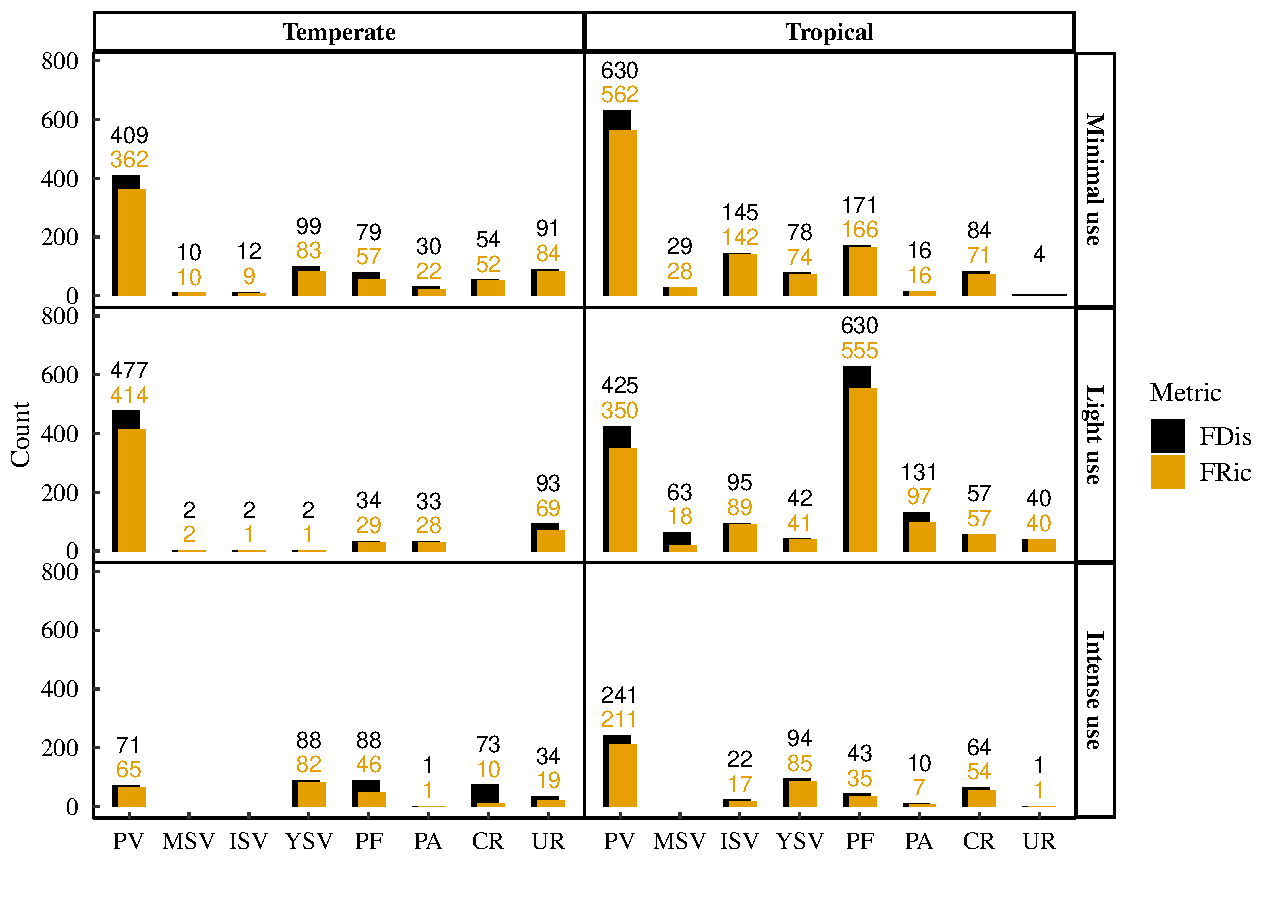
\includegraphics[scale=0.8]{Supporting/Chapter3/Figures/SI_samplesizes}
\caption[Number of sites in each land use and use intensity for which FRic and FDis were calculated, across all species]{\textbf{Number of sites in each land use and use intensity for which FRic and FDis were calculated, across all species.} The number of sites for FRic can be smaller than the number of sites for FDis because FRic could not necessarily be computed for all assemblages in which FDis was estimated (in assemblages where species richness was 2 or 3, FRic could not be computed).}
\label{SI3_F1}
\end{figure}

\pagebreak

\begin{figure}[h!]
\centering
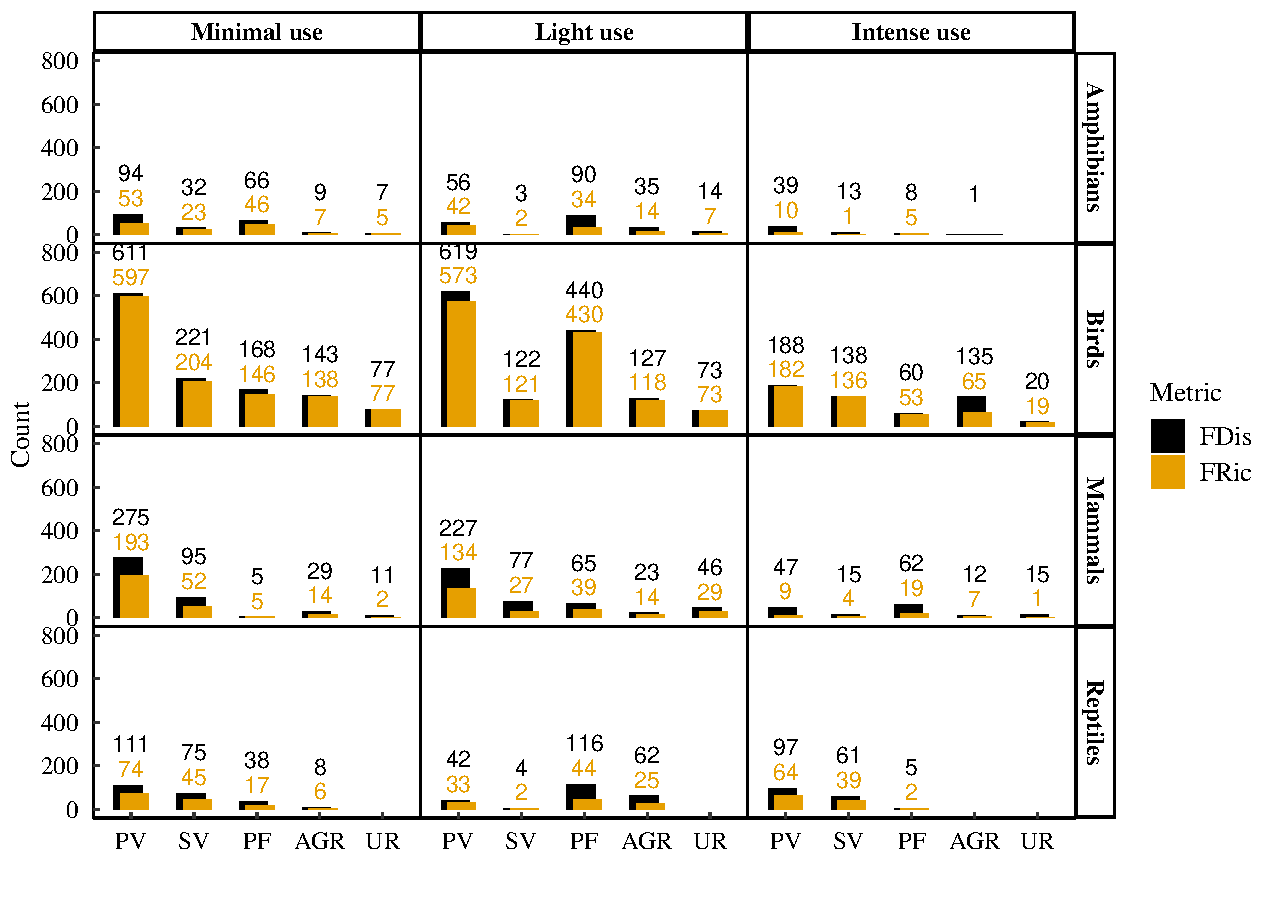
\includegraphics[scale=0.8]{Supporting/Chapter3/Figures/SI_samplesizes_fig3}
\caption[Number of sites in each land use, use intensity and for which FRic and FDis were calculated, within each class]{\textbf{Number of sites in each land use, use intensity and for which FRic and FDis were calculated, within each class.} The number of sites for FRic can be smaller than the number of sites for FDis because FRic could not necessarily be computed for all assemblages in which FDis was estimated (in assemblages where species richness was 2 or 3, FRic could not be computed).}
\label{SI3_F2}
\end{figure}

\pagebreak
\clearpage

\section{Trait data \& imputation of missing trait values}

We used a compilation of trait data across terrestrial vertebrates (Chapter 2; \citet{Etard2020}). We used seven traits that were available at least for a subset of the species in each class: body mass, trophic level, lifespan, litter/clutch size, diel activity, habitat breadth and use of artificial habitats. These traits related to life-history, habitat specialisation and use of geographical space (for instance, habitat breadth is a significant predictor of geographical range size in all classes, Fig. \ref{}). 

%% Habitat breadth predicts range size
\begin{figure}[h!]
\centering
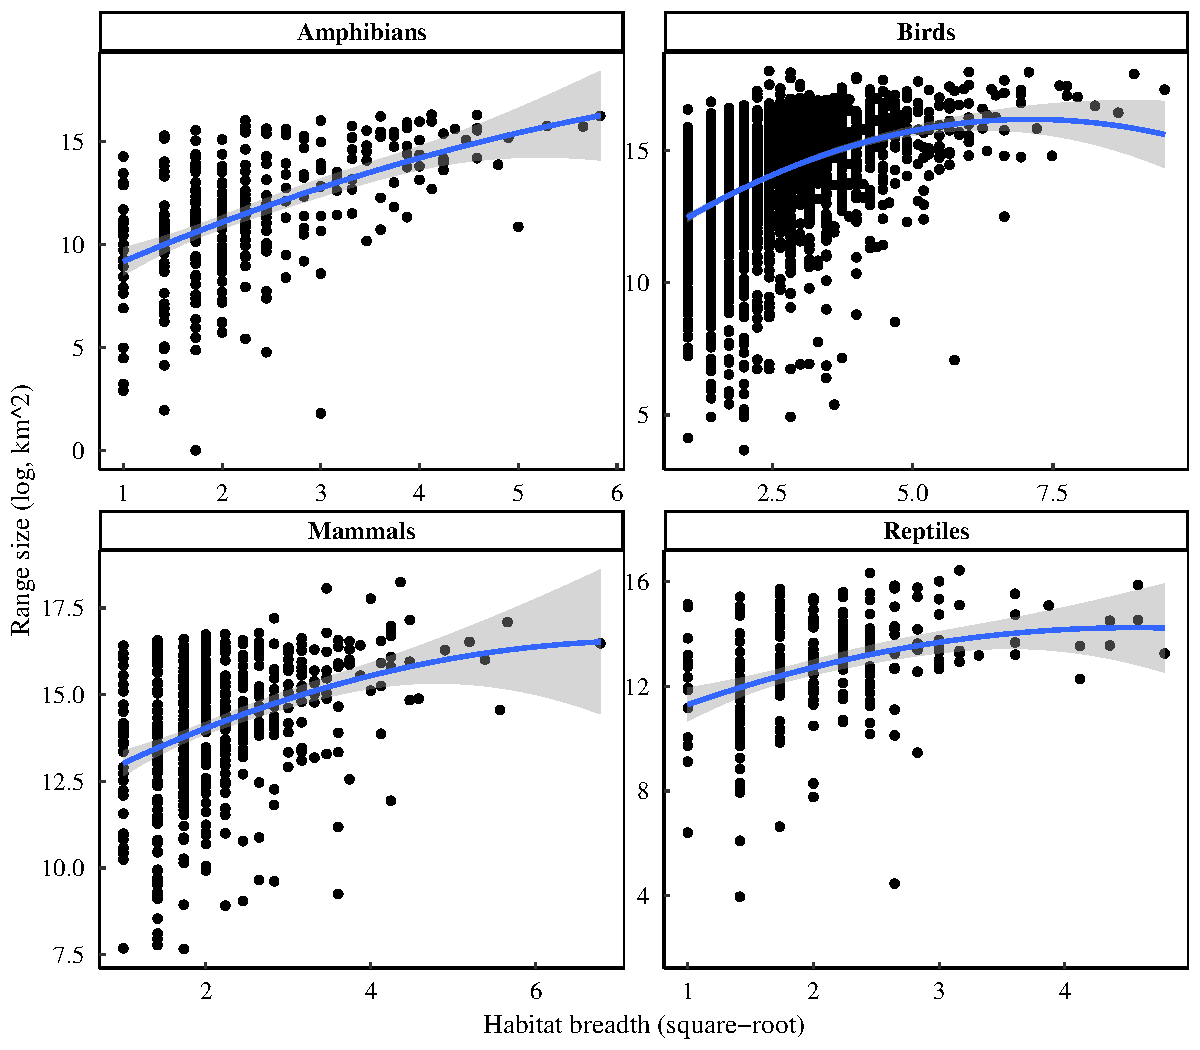
\includegraphics[scale=0.6]{Supporting/Chapter3/Figures/SI_Rangesize_HB}
\caption[Relationship between habitat breadth and geographical range size across species in each class]{\textbf{Relationship between habitat breadth and geographical range size across species in each class.} The derivation of geographical range sizes is described in Chapter 2.}
\label{SI3_F3}
\end{figure}

Trait-data coverage was highly variable among classes and traits, with important geographical and phylogenetic biases in trait data for reptiles and amphibians (\cite{Etard2020}; Fig. S4, Fig. S5). To obtain complete species-trait datasets, we imputed missing trait values. Further, in order to assess the sensitivity of our models to variation in imputed values, we imputed the missing trait values eight independent times. This allowed us to assess the congruence of our model predictions when using the different imputed trait datasets in the analyses. 

%% Trait coverage
\begin{figure}[h!]
\centering
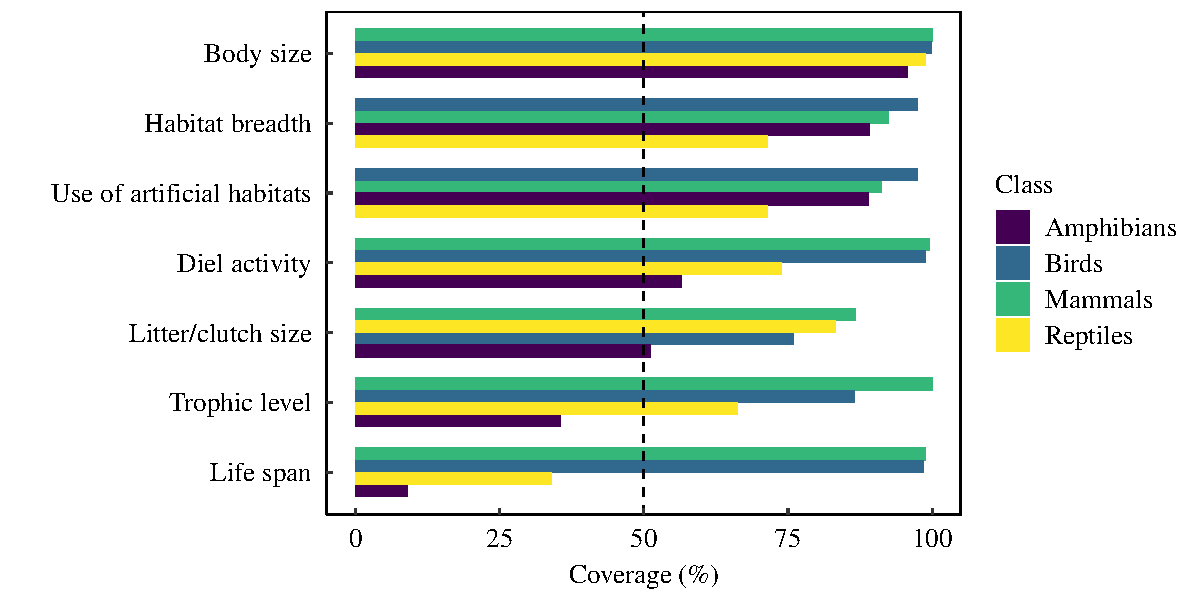
\includegraphics[scale=0.8]{Supporting/Chapter3/Figures/SI_coverage}
\caption[Trait coverage for the vertebrate species sampled in the PREDICTS database]{\textbf{Trait coverage for the vertebrate species sampled in the PREDICTS database.} For a given trait, coverage is calculated as the percentage of species for which an estimate was available.}
\label{SI3_F4}
\end{figure}

%% Trait completeness
\begin{figure}[h!]
\centering
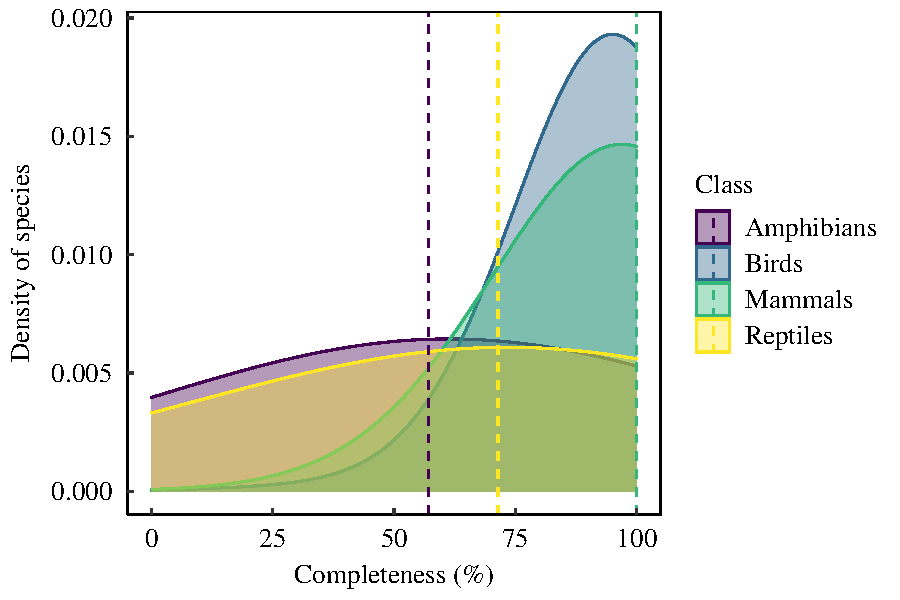
\includegraphics[scale=0.8]{Supporting/Chapter3/Figures/SI_completeness}
\caption[Distribution of trait completeness across the vertebrate species sampled in the PREDICTS database]{\textbf{Distribution of trait completeness across the vertebrate species sampled in the PREDICTS database.} For a given species, trait completeness is calculated as the proportion of traits for which an estimate was available. Dashed lines represent the median trait completeness.}
\label{SI3_F5}
\end{figure}


\clearpage

\subsection{Choice of imputation technique}
There exist several imputation techniques \citep{Etard2020, Penone2014, Debastiani2021, Johnson2021}, such as K-nearest neighbour \citep{Troyanskaya2001}, multivariate imputation by chained equations \citep{micepackage}, random forest algorithms (implementable in R with missForest; \cite{Stekhoven2012, Stekhoven2016}), and phylogenetic imputations (implementable in R with PhyloPars, \cite{Bruggeman2009}). \citet{Penone2014} assessed the performance of these four techniques and showed that missForest and PhyloPars performed better when traits were phylogenetically conserved, and when the species phylogenetic position was included as a predictor of missing trait values. PhyloPars can only handle continuous data, while missForest is compatible with mixed-type (including categorical) data. When no phylogenetic information was included, mice was found to be the best method, with fast imputations of mixed-type data \citep{Penone2014}. Therefore, to assess whether missForest or mice was more appropriate here, we measured the phylogenetic signal in trait data. For continuous traits, we used Pagel’s $\lambda$ \citep{Pagel1999}, and for categorical traits we used Borges’ $\delta$ \citep{Borges2018}. Strong phylogenetic signal would indicate that traits are phylogenetically conserved, and hence missForest would be the most suited approach for imputing missing trait values, with the inclusion of species’ phylogenetic positions as a predictor. 

\subsection{Phylogenetic signal in traits}
Across all classes, similar traits were used for calculating functional diversity metrics: body mass, litter/clutch size, lifespan (using different proxies in different vertebrate classes: generation length for birds and mammals, longevity for reptiles, and age at sexual maturity for amphibians), trophic level, diel activity, habitat breadth and use of artificial habitats. In addition, we included some class-specific traits for the imputations, as certain class-specific traits could be useful predictors of other traits (such as body length for instance in amphibians \citep{Santini2018}). Table S2 details the traits that were included for the imputations in each class and the phylogenetic signal for each of these traits. Continuous traits were log-10 transformed before assessing Pagel’s $\lambda$ to improve normality. Pagel’s $\lambda$ was estimated using the phylosig function of the phytools package \citep{Revell2012}, and Borges’ $\delta$ was assessed using code provided by \citet{Borges2018}, available at : \url{https://github.com/mrborges23/delta_statistic}. To test for the significance of $\delta$, we generated null distributions of $\delta$ for each categorical trait by randomising trait vectors 50 times, and calculating $\delta$ for each randomised vector – following the guidelines proposed by \citet{Borges2018}. We then tested whether the observed medians were greater than the null distributions using one-sided Wilcoxon rank sum tests.

We used class-specific phylogenies to estimate phylogenetic signal, all downloaded on 13th April 2020. Trees from \citet{Faurby2018, Faurby2020}  were used for mammals (downloaded from \url{https://zenodo.org/record/3690867#.Xyc5wyhKhPZ}). For amphibians, birds and reptiles (squamates only), we downloaded trees from \url{https://data.vertlife.org/}. Trees were from \citet{Jetz2012} for birds, from \citet{Jetz2018} for amphibians and from \citet{Tonini2016} for squamates. For each class, we downloaded a distribution of 1,000 trees, from which we obtained consensus trees to estimate phylogenetic signal (to that end, we used the TreeAnnotator programme of the BEAST software \citep{Bouckaert2014}).


\begin{table}[h!]
\renewcommand{\baselinestretch}{1}
\renewcommand{\arraystretch}{1.2}
\begin{center}\fontsize{9}{11}\selectfont
\caption[Phylogenetic signal in continuous and categorical traits]{\textbf{Phylogenetic signal in continuous and categorical traits.} BM: body mass; BL: body length; GL: generation length; MA: age at sexual maturity; ML: maximum longevity; L: longevity; LCS: litter/clutch size; HB: habitat breadth; TL: trophic level; DA: diel activity; UA: use of artificial habitats. Continuous traits were log-10 transformed to improve normality before estimating Pagel’s $\lambda$ – except for habitat breadth which was square-rooted. A star indicates a significant signal (p-value<0.05 for the log-likelihood ratio test in the case of $\lambda$; and a significant difference from the simulated null distribution of $\delta$ for categorical traits). ‘NA’ indicates traits that were not considered for a given class. All traits showed significant phylogenetic signal, with signals for BM, BL, L, GL, MA and LCS being particularly strong (above 0.8) across the four classes. }
\label{SI3_Table2}  
\begin{tabular}{l|c|c|c|c|c|c|c|c|c|c|c|}
\cline{2-12}
                                          & \multicolumn{8}{c|}{\textbf{Pagel's $\lambda$}}                                                                       & \multicolumn{3}{c|}{\textbf{Borges' $\delta$}} \\ \hline
\multicolumn{1}{|c|}{\textbf{Class}}      & \textbf{BM} & \textbf{BL} & \textbf{GL} & \textbf{MA} & \textbf{ML} & \textbf{L} & \textbf{LCS} & \textbf{HB} & \textbf{TL} & \textbf{DA} & \textbf{UA} \\ \hline
\multicolumn{1}{|l|}{\textbf{Amphibians}} & 0.98*       & 0.94*       & NA          & 0.85*       & 0.82*       & NA         & 0.93*        & 0.99*       & 18*         & 3.4*        & 4.5*        \\ %\hline
\multicolumn{1}{|l|}{\textbf{Birds}}      & 0.99*       & NA          & 0.97*       & NA          & NA          & NA         & 0.95*        & 0.60*       & 13*         & 32e3*       & 1.8*        \\ %\hline
\multicolumn{1}{|l|}{\textbf{Mammals}}    & 0.99*       & NA          & 0.97        & NA          & NA          & NA         & 0.99         & 0.71        & 26*         & 17*         & 1.3*        \\ %\hline
\multicolumn{1}{|l|}{\textbf{Reptiles}}   & 1.0*        & NA          & NA          & NA          & 0.94*       & 0.98*      & 1.0*         & 0.52*       & 6.3*        & 6.4*        & 1.4*        \\ \hline
\end{tabular}
\end{center}
\end{table}

\subsection{Implementation of missForest imputations}
As phylogenetic signals were strong in many categorical and continuous traits (Table \ref{}), we imputed missing trait values using random forest algorithms, as implemented in R with missForest \citep{Stekhoven2012, Stekhoven2016}. Another advantage of missForest was that, being a non-parametric approach, no prior assumption about data distribution was required. The data were therefore not transformed prior to imputations. In addition, \citet{Penone2014} showed that including phylogenetic information did not decrease the accuracy of imputations for traits that were less phylogenetically conserved, such as habitat breadth in this work. 

Phylogenetic relationships were included as additional predictors in the form of phylogenetic eigenvectors \citep{DinizFilho2012}, extracted from the phylogenies using the PVR package \citep{Santos2018}. Following \citet{Penone2014}, we included the first ten phylogenetic eigenvectors as additional predictors of missing trait values in each class, enough to minimise imputation error. As not all species were represented in the phylogenies, we also added taxonomic order as a predictor for all species. All traits in Table S2 were included in the imputations. Tuning parameters of missForest were set to ten maximum iterations and to one hundred trees grown in each forest. 

\section{Degree of multicollinearity among traits}
Multicollinearity among traits can be problematic when calculating functional diversity indices \citep{Cadotte2011}. After imputing missing trait values and before estimating functional metrics, we hence assessed whether the degree of multicollinearity among categorical and continuous traits was not problematically high. To that end, we used generalised variance inflation factors \citep{Fox1992}. Given a regression model, variance inflation factors quantify the overestimation in the variance of estimated regression coefficients due to multicollinearity among the predictors. A GVIF value of 5 or 10 is commonly used as a threshold to select out collinear predictors \citep{Dormann2013}. We used the stepwise.vif function of the Rnalytica package (\url{https://github.com/awsm-research/Rnalytica}), with a threshold of 5, to determine the GVIF of each trait. We used the imputed traits from the 8th imputation iteration to assess whether multicollinearity was problematically high. Continuous traits were log-10 transformed (except for habitat breadth which was square-rooted). Multicollinearity across traits was not detected to be problematically high, as all traits had a GVIF value below 2 (Table S3). As such, all seven traits were included in the calculation of functional diversity indices.

\begin{table}[h!]
\renewcommand{\baselinestretch}{1}
\renewcommand{\arraystretch}{1.2}
\begin{center}\fontsize{9}{11}\selectfont
\caption[Variance inflation factors across considered (imputed) traits]{\textbf{Variance inflation factors across considered (imputed) traits.}} 
\label{SI3_Table3}  
\begin{tabular}{|l|c|}
\hline
\textbf{Trait}                & \multicolumn{1}{l|}{\textbf{GVIF}} \\ \hline
Diel activity                 & 1.1                                \\ 
Trophic level                 & 1.3                                \\ 
Use of artificial habitats    & 1.4                                \\
Body mass (log10)             & 1.5                                \\ 
Habitat breadth (square-root) & 1.5                                \\ 
Litter/clutch size (log10)    & 1.6                                \\ 
Lifespan proxy (log10)        & 1.7                                \\ \hline
\end{tabular}
\end{center}
\end{table}

\newpage

\section{Imputation performance}

%% Trait distirubtion (continuous) before and after imputation
\begin{figure}[h!]
\centering
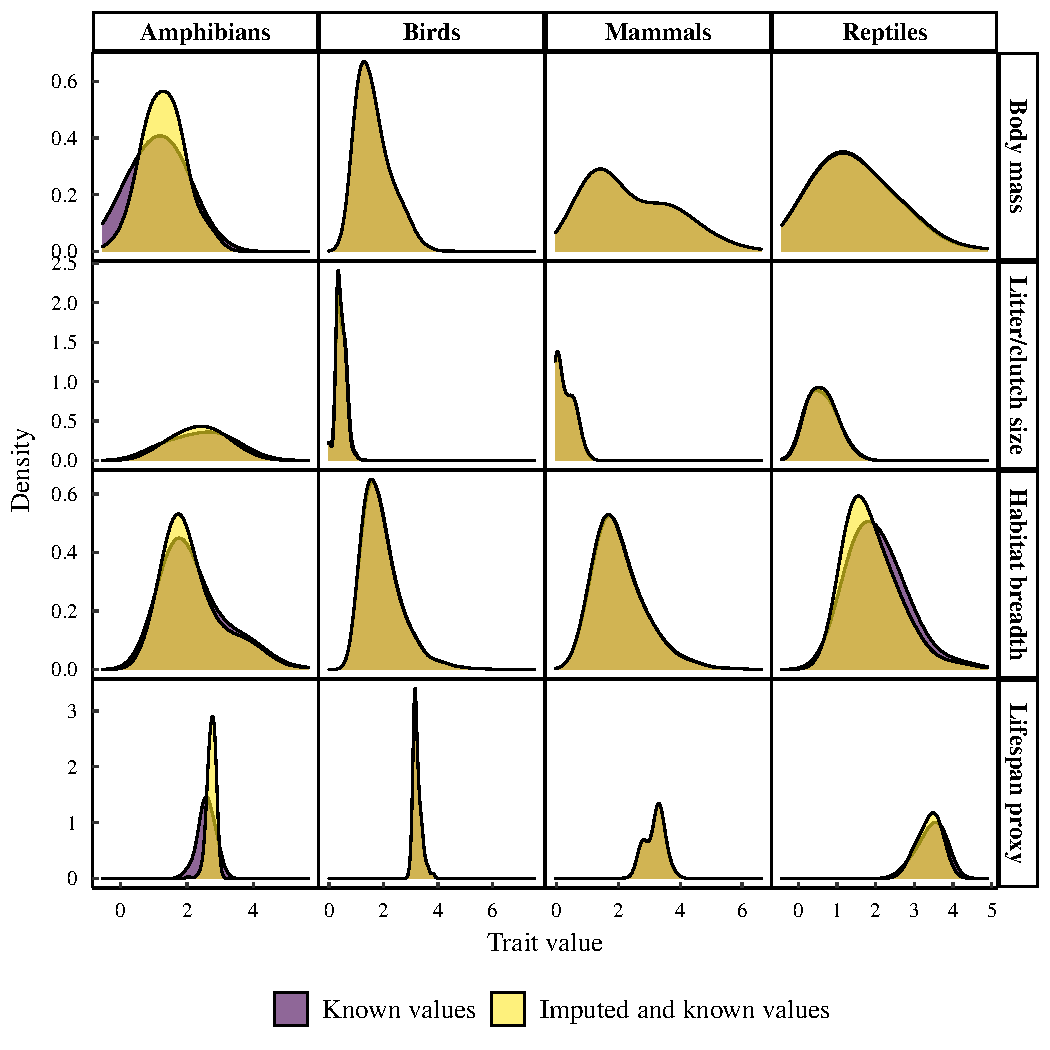
\includegraphics[scale=0.8]{Supporting/Chapter3/Figures/SI_dist_cont}
\caption[Distribution of continuous traits considered in the calculation of the functional diversity metrics]{\textbf{Distribution of continuous traits considered in the calculation of the functional diversity metrics (shown as density plots), before and after missing value imputations, in each class and for the species occurring in the PREDICTS database.} All traits were log10-transformed except Habitat breadth, which was square-rooted.}
\label{SI3_F6}
\end{figure}

\newpage
%% Trait distirubtion (categorical) before and after imputation
\begin{figure}[h!]
\centering
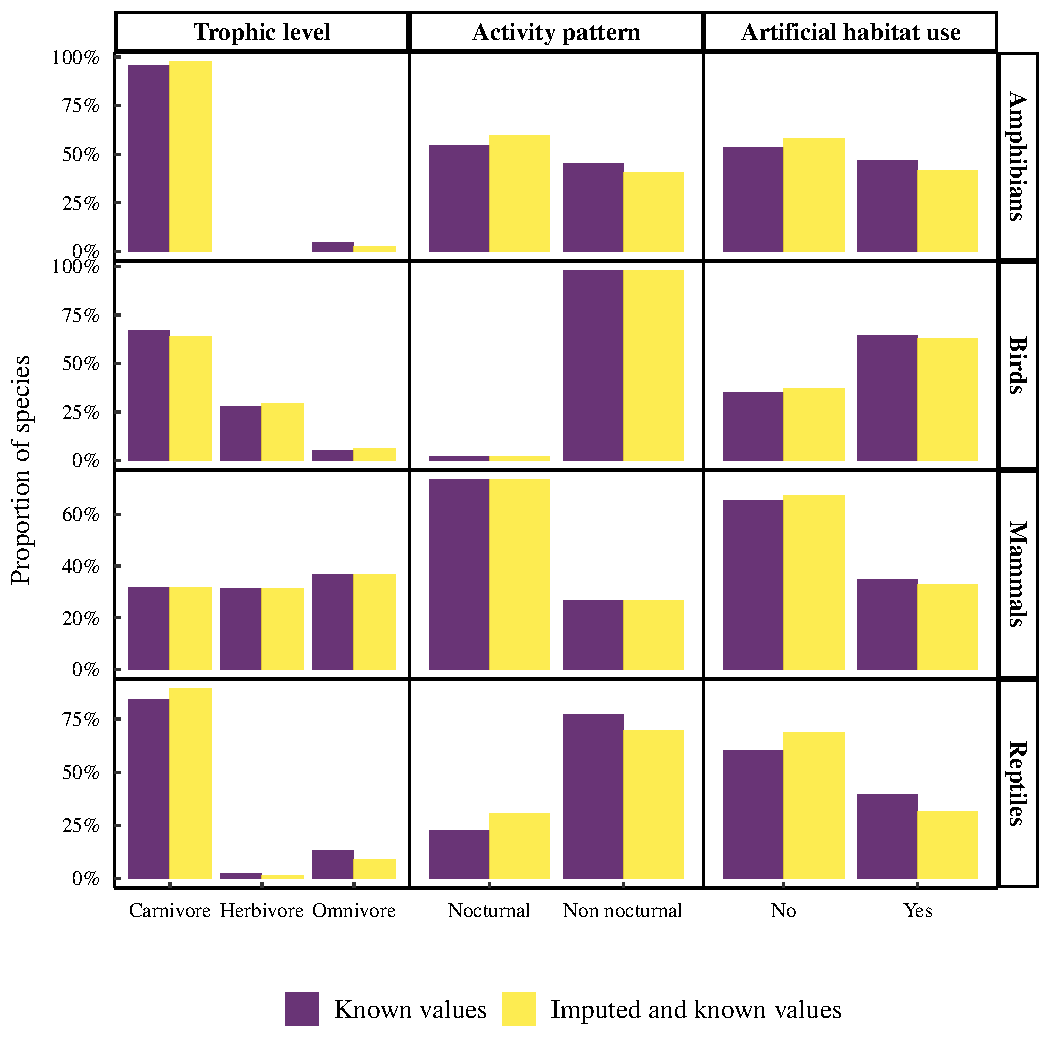
\includegraphics[scale=0.8]{Supporting/Chapter3/Figures/SI_dist_cat}
\caption[Frequency distribution for categorical traits considered in the calculation of the functional diversity metrics]{\textbf{Frequency distribution for categorical traits considered in the calculation of the functional diversity metrics (shown as \% of total species in each category) before and after missing value imputations, in each class, for the species occurring in the PREDICTS database.}}
\label{SI3_F7}
\end{figure}
\newpage

%% Imputation error
\begin{figure}[h!]
\centering
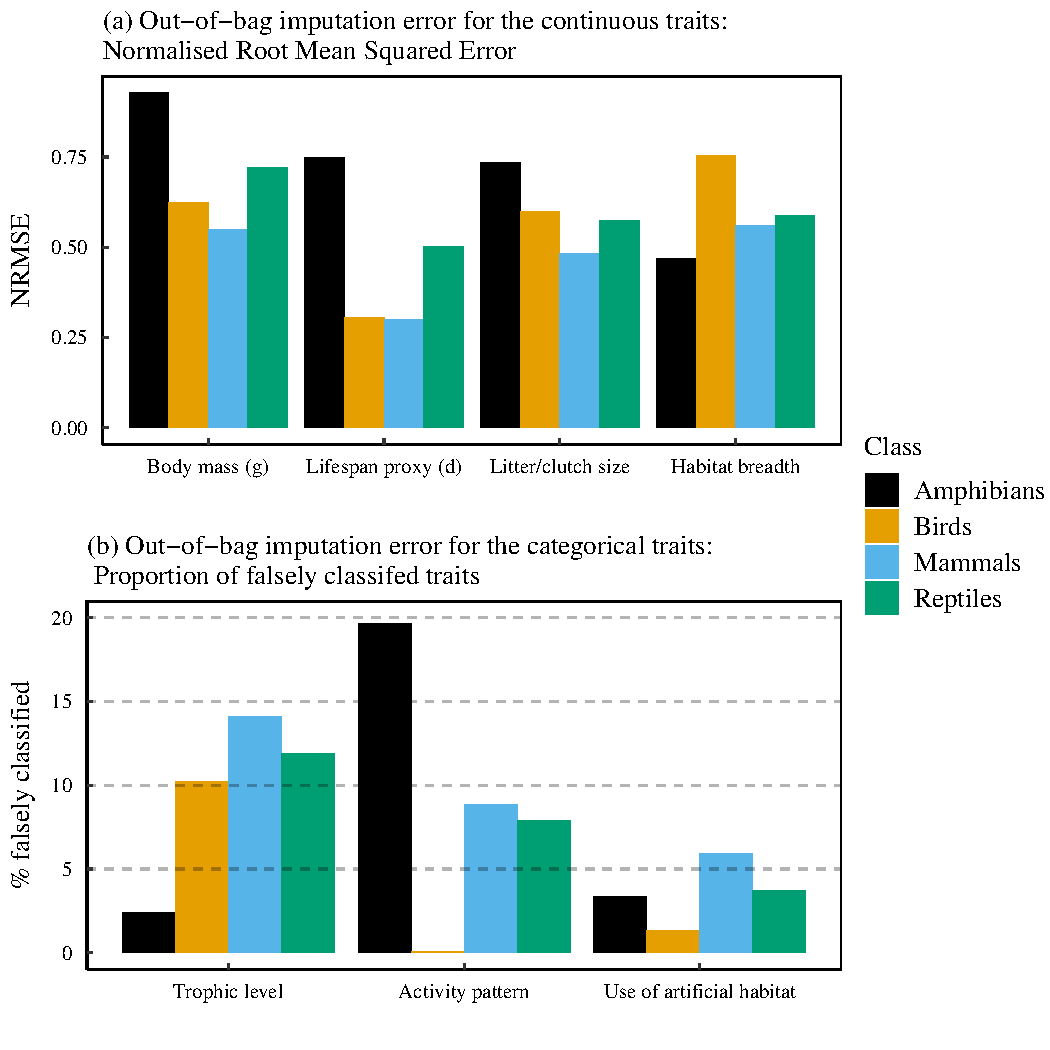
\includegraphics[scale=0.8]{Supporting/Chapter3/Figures/SI_imputation_errors}
\caption[Out-of-bag imputation errors for the continuous traits (a) and categorical traits (b)]{\textbf{Out-of-bag imputation errors for the continuous traits (a) and categorical traits (b).} For continuous traits, the Normalised Root Mean Squared Error (NRMSE) was obtained by dividing the Mean Squared Error (MSE) by the variance of the known trait distribution, then square-rooting the result. The MSE was returned for each trait by the missforest function (missForest package, \cite{Stekhoven2012, Stekhoven2016}) and corresponds to an out-of-bag error. For categorical traits, the error was estimated as the out-of-bag proportion of falsely classified traits.}
\label{SI3_F8}
\end{figure}

\newpage

\section{Functional loss and functional gain}

Across all vertebrates, we estimated functional loss and gain using 84 studies for the tropical subset and 39 studies for the temperate subset (51,514 and 30,470 pairwise comparisons between sites respectively, Table S4). Because of this large number of pairwise comparisons, we did not develop a null modelling approach (if we used 100 randomisations per pair of sites, we would need to compute functional loss and gain for more than 8 million pairs, which would be very computationally demanding). We grouped mature, intermediate and young secondary vegetation together in this analysis. We could not estimate the effects in all land uses (for instance, sample sizes for tropical urban sites were too small).

Within classes, we used 18 tropical studies and 1 temperate study for amphibians; 38 and 21 for birds (respectively); 28 and 9 for mammals; and 11 and 7 for reptiles. As sample sizes differed among pairs of land uses and use intensities (Table S5), we were not able to estimates all effects, notably for the intensely-used land uses. 

To calculate functional loss and functional gain, the Gower distance matrix was first subsetted to the species occurring in a given pair of sites (see main text, Material and Methods, `Functional diversity indices'). Cailliez corrections were applied when the distance matrix was not Euclidian (Cailliez corrections consist of applying the smallest positive constant to the distances so as to make them Euclidian \citep{Cailliez1983}; ade4 R package \citep{ade4package}). We then performed a principal coordinates analysis on the (corrected) Gower distance matrix, retaining the first two axes to reduce the computational load in the calculation of convex hulls. Sites that contained fewer than three functionally different species were excluded (the computation of a convex hull requiring more species in the assemblage than PCoA axes). Then we estimated the volume of trait space occupied by each assemblage of a given pair, as well as the volume of the shared trait space (intersection), from which we derived functional loss and functional gain.

\vspace{1cm}
\begin{table}[h!]
\renewcommand{\baselinestretch}{1}
\renewcommand{\arraystretch}{1.2}
\begin{center}\fontsize{9}{11}\selectfont
\caption[Sample sizes (number of pairs of sites) for the calculation of functional loss and functional gain across all species]{\textbf{Sample sizes (number of pairs of sites) for the calculation of functional loss and functional gain across all species.}} 
\label{SI3_Table4}  
\begin{tabular}{@{\extracolsep{5pt}} cccccc} 
\\[-1.8ex]\hline 
\textbf{Region}            & \textbf{Pairs} & \textbf{Minimal use} & \textbf{Light use} & \textbf{Intense use} \\ \hline
\multirow{6}{*}{Temperate} & PV-PV          & 7626                 & 22546              & 492                  \\
                           & PV-SV          & 511                  & 72                 & --                   \\
                           & PV-PF          & 9                    & 166                & --                   \\
                           & PV-PA          & 8                    & 40                 & --                   \\
                           & PV-CR          & 150                  & --                 & --                   \\
                           & PV-UR          & 6306                 & 1197               & 7                    \\ \hline
\multirow{6}{*}{Tropical}  & PV-PV          & 8547                 & 4016               & 16722                \\
                           & PV-SV          & 6584                 & 1124               & 9713                 \\
                           & PV-PF          & 580                  & 1378               & --                   \\
                           & PV-PA          & 36                   & 20                 & 22                   \\
                           & PV-CR          & 1700                 & 1088               & --                   \\
                           & PV-UR          & --                   & --                 & --                   \\ \hline
\end{tabular}
\end{center}
\end{table}

\clearpage
\newpage

%% sample sizes by class
% Table created by stargazer v.5.2.2 by Marek Hlavac, Harvard University. E-mail: hlavac at fas.harvard.edu
% Date and time: Tue, Jun 22, 2021 - 11:31:53
\begin{table}[!htbp]
\renewcommand{\baselinestretch}{1}
\renewcommand{\arraystretch}{1.2}
\begin{center}\fontsize{9}{11}\selectfont
  \caption[Sample sizes (number of pairs of sites) for the calculation of functional loss and functional gain within each class]{\textbf{Sample sizes (number of pairs of sites) for the calculation of functional loss and functional gain within each class.}}
  \label{SI3_Table5} 
\begin{tabular}{@{\extracolsep{5pt}} cccccc} 
\\[-1.8ex]\hline 
\hline \\[-1.8ex] 
\textbf{Class} & \textbf{Region} & \textbf{Pair of land uses} & \textbf{Minimal use} & \textbf{Light use} & \textbf{Intense use}\\ 
\hline \\[-1.8ex] 
Amphibians & Temperate & PV/PV & -- & 45 & -- \\ 
Amphibians & Temperate & PV/SV & 8 & 70 & -- \\ 
Amphibians & Temperate & PV/AGR & 3 & -- & -- \\ 
Amphibians & Temperate & PV/UR & 6 & 100 & -- \\ 
Amphibians & Tropical & PV/PV & 501 & 241 & 307 \\ 
Amphibians & Tropical & PV/SV & 838 & -- & 90 \\ 
Amphibians & Tropical & PV/PF & 422 & 91 & -- \\ 
Amphibians & Tropical & PV/AGR & 1 & 3 & 1 \\ 
Birds & Temperate & PV/PV & 7,382 & 19,300 & 491 \\ 
Birds & Temperate & PV/SV & 150 & 1 & -- \\ 
Birds & Temperate & PV/PF & 9 & 166 & -- \\ 
Birds & Temperate & PV/AGR & 145 & 40 & -- \\ 
Birds & Temperate & PV/UR & 6,300 & 992 & -- \\ 
Birds & Tropical & PV/PV & 5,059 & 3,117 & 9,014 \\ 
Birds & Tropical & PV/SV & 3,491 & 1,058 & 5,225 \\ 
Birds & Tropical & PV/PF & 156 & 994 & -- \\ 
Birds & Tropical & PV/AGR & 1,626 & 1,085 & -- \\ 
Mammals & Temperate & PV/PV & 110 & 3,030 & -- \\ 
Mammals & Temperate & PV/SV & 25 & -- & -- \\ 
Mammals & Temperate & PV/AGR & 5 & -- & -- \\ 
Mammals & Temperate & PV/UR & -- & 105 & 7 \\ 
Mammals & Tropical & PV/PV & 1,989 & 637 & 64 \\ 
Mammals & Tropical & PV/SV & 230 & 65 & 8 \\ 
Mammals & Tropical & PV/PF & 2 & -- & -- \\ 
Mammals & Tropical & PV/AGR & 109 & 20 & 21 \\ 
Reptiles & Temperate & PV/PV & 132 & 2 & 1 \\ 
Reptiles & Temperate & PV/SV & 250 & 1 & -- \\ 
Reptiles & Temperate & PV/AGR & 5 & -- & -- \\ 
Reptiles & Tropical & PV/PV & 989 & 137 & 5,140 \\ 
Reptiles & Tropical & PV/SV & 1,760 & 1 & 3,456 \\ 
Reptiles & Tropical & PV/PF & -- & 190 & -- \\ 
\hline \\[-1.8ex] 
\end{tabular}
\end{center} 
\end{table} 

\clearpage
\newpage

\section{Diagnostic plots}


% Model 1a
%% diagnostic plots for model FRic across ter ver
\begin{figure}[h!]
\centering
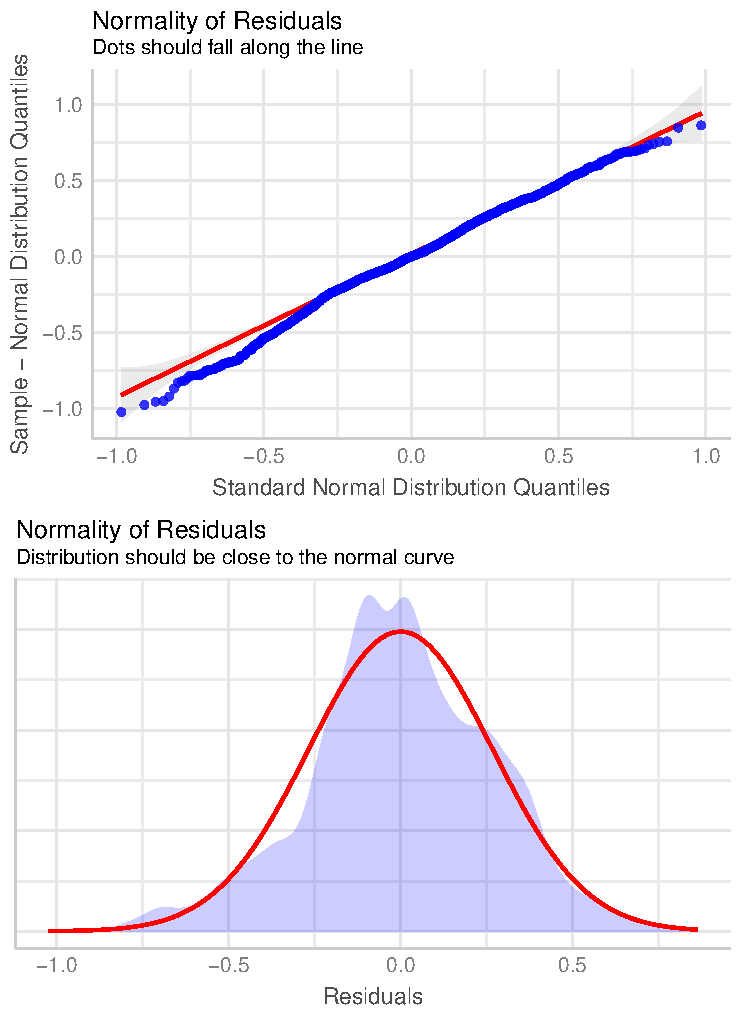
\includegraphics[scale=0.7]{Supporting/Chapter3/Figures/Diagnostics/SI_diagnostics_Model1a}
\caption[Diagnostic plots for Model 1a]{\textbf{Diagnostic plots for \underline{Model 1a},} obtained using the `performance' R package \citep{performance}.}
\label{SI3_F9}
\end{figure}

\newpage

% Model 1b
%% diagnostic plots for model FDis across ter ver
\begin{figure}[h!]
\centering
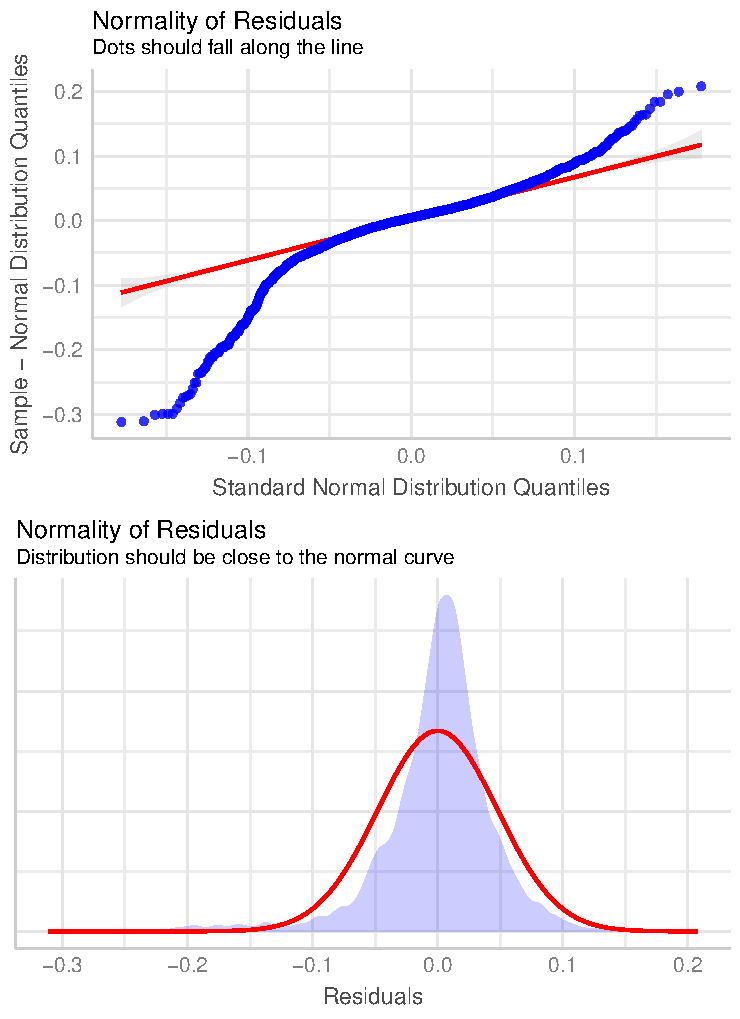
\includegraphics[scale=0.7]{Supporting/Chapter3/Figures/Diagnostics/SI_diagnostics_Model1b}
\caption[Diagnostic plots for Model 1b]{\textbf{Diagnostic plots for \underline{Model 1b},} obtained using the `performance' R package \citep{performance}.}
\label{SI3_F10}
\end{figure}

\newpage

% Model 2a
\begin{figure}[h!]
\centering
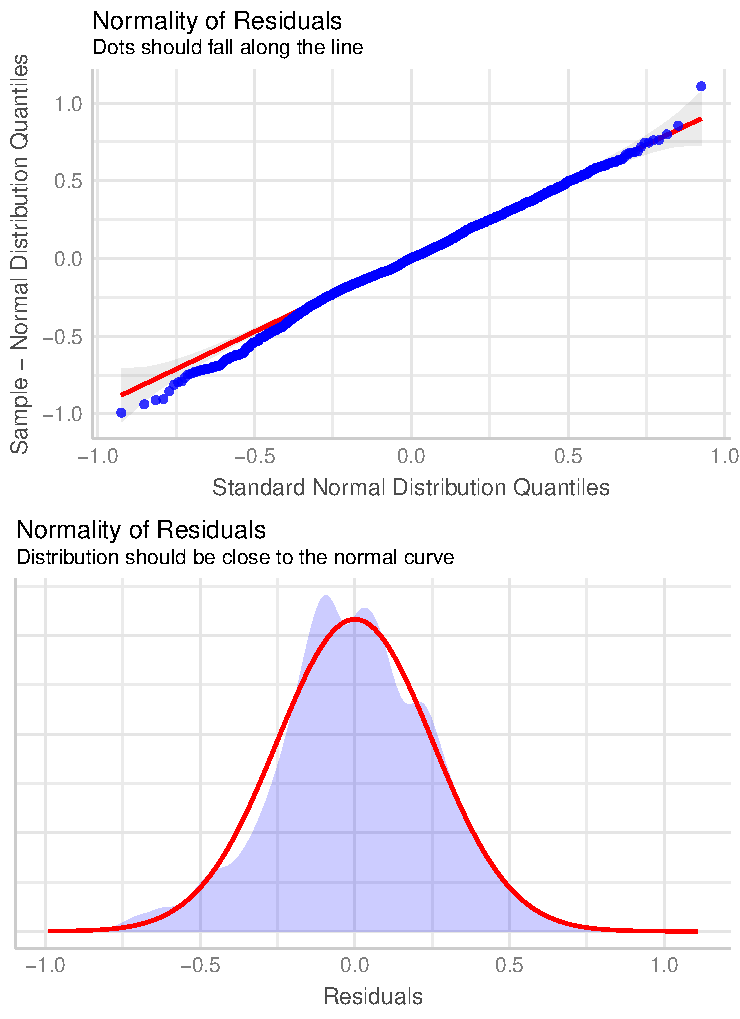
\includegraphics[scale=0.7]{Supporting/Chapter3/Figures/Diagnostics/SI_diagnostics_Model2a}
\caption[Diagnostic plots for Model 2a]{\textbf{Diagnostic plots for \underline{Model 2a},} obtained using the `performance' R package \citep{performance}.}
\label{SI3_F11}
\end{figure}

\newpage

% Model 2b
\begin{figure}[h!]
\centering
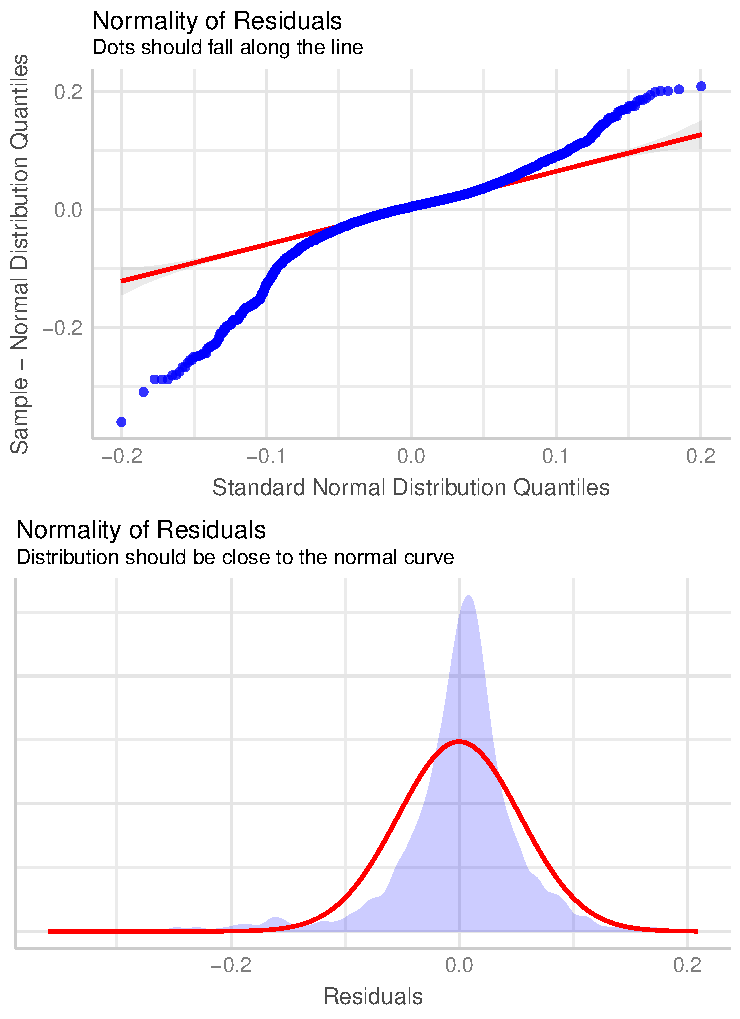
\includegraphics[scale=0.7]{Supporting/Chapter3/Figures/Diagnostics/SI_diagnostics_Model2b}
\caption[Diagnostic plots for Model 2b]{\textbf{Diagnostic plots for \underline{Model 2b},} obtained using the `performance' R package \citep{performance}.}
\label{SI3_F12}
\end{figure}

\newpage

% Model 3
%% diagnostic plots for binomial model (DHarma)
\begin{figure}[h!]
\centering
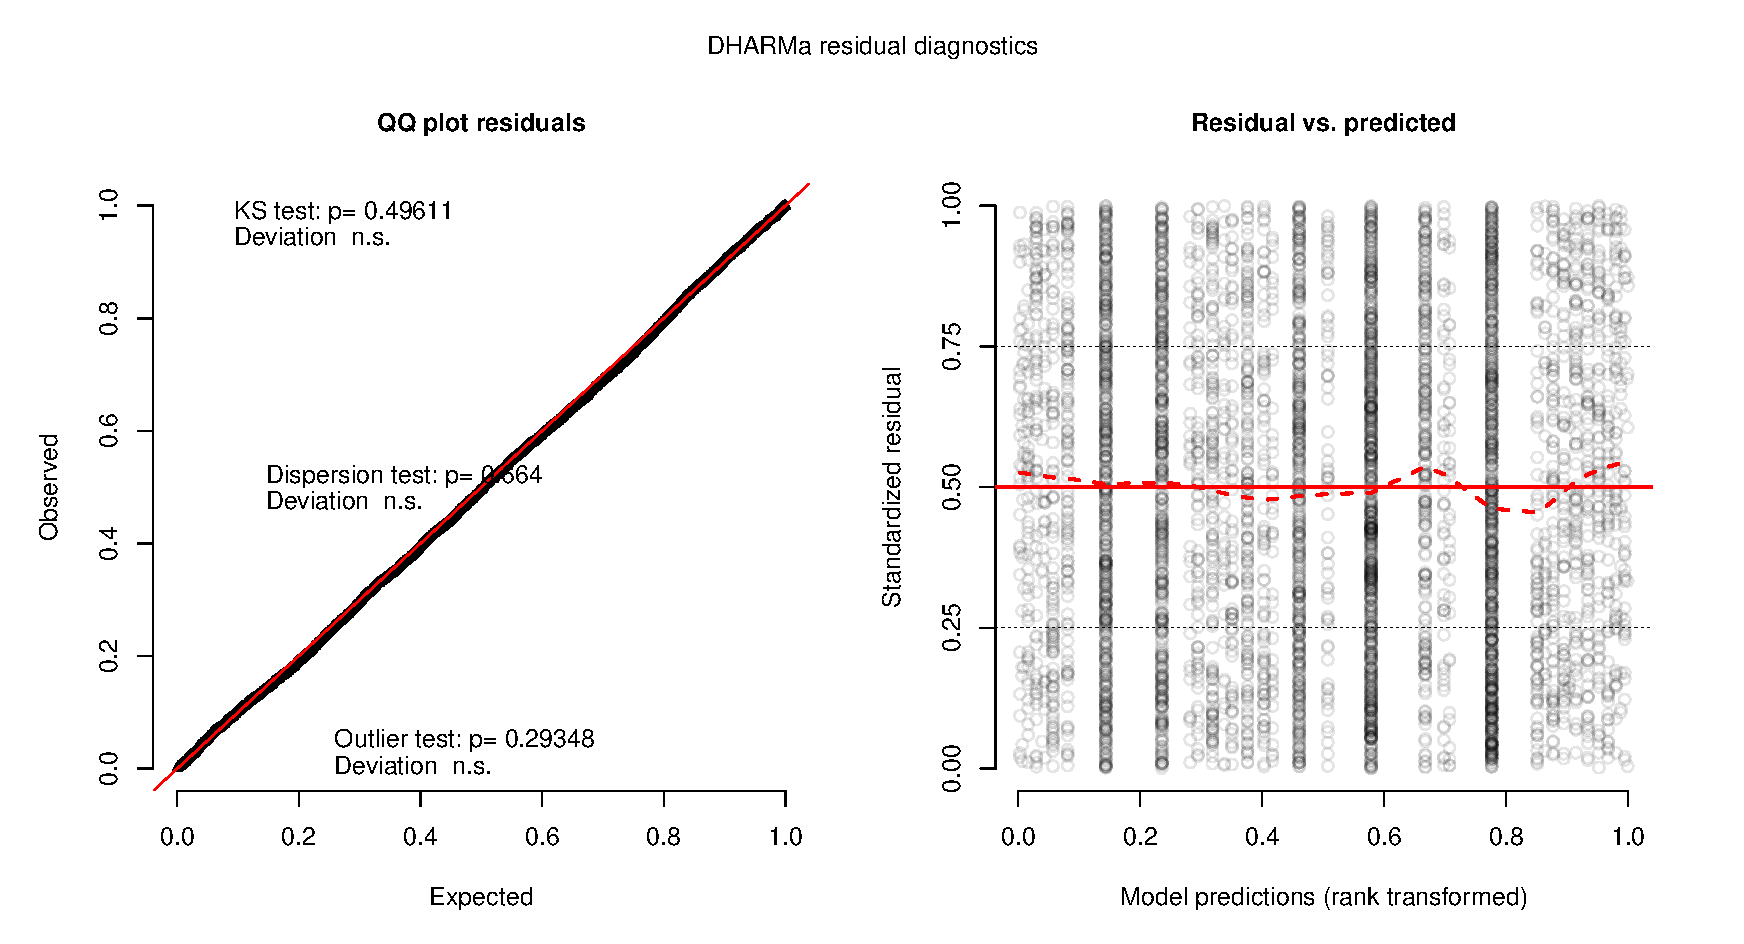
\includegraphics[scale=0.6]{Supporting/Chapter3/Figures/Diagnostics/SI_diagnostics_Model3}
\caption[Diagnostic plots for Model 3]{\textbf{Diagnostic plots for \underline{Model 3},} obtained using the `DHARMa' R package \citep{DHARMa}.}
\label{SI3_F13}
\end{figure}

\newpage


% Model 4a
\begin{figure}[h!]
\centering
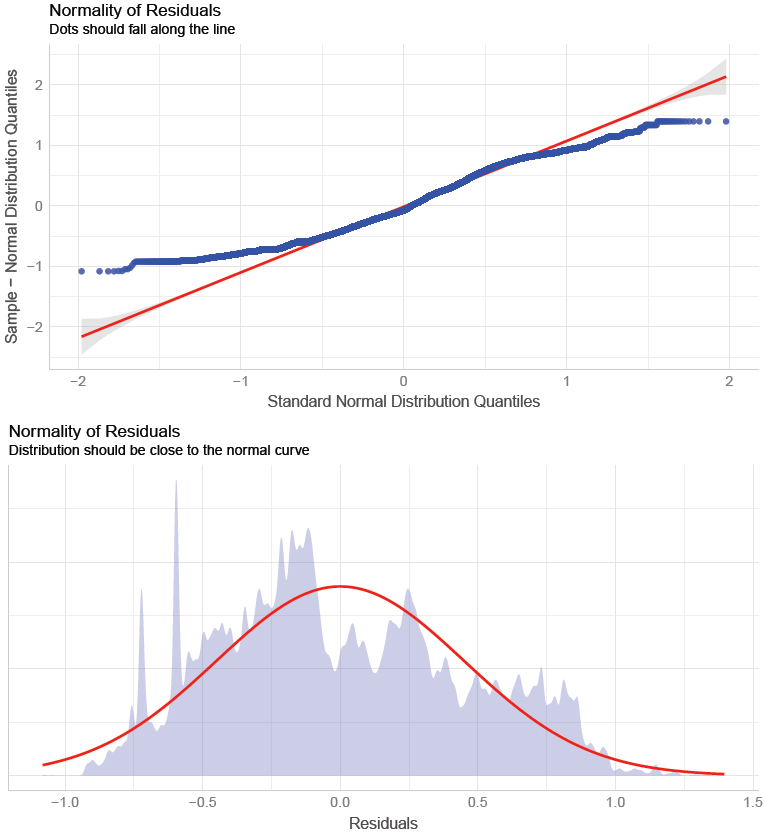
\includegraphics[scale=0.7]{Supporting/Chapter3/Figures/Diagnostics/Diag_model_4a}
\caption[Diagnostic plots for Model 4a]{\textbf{Diagnostic plots for \underline{Model 4a},} obtained using the `performance' R package \citep{performance}.}
\label{SI3_F14}
\end{figure}

\newpage

% Model 4b
\begin{figure}[h!]
\centering
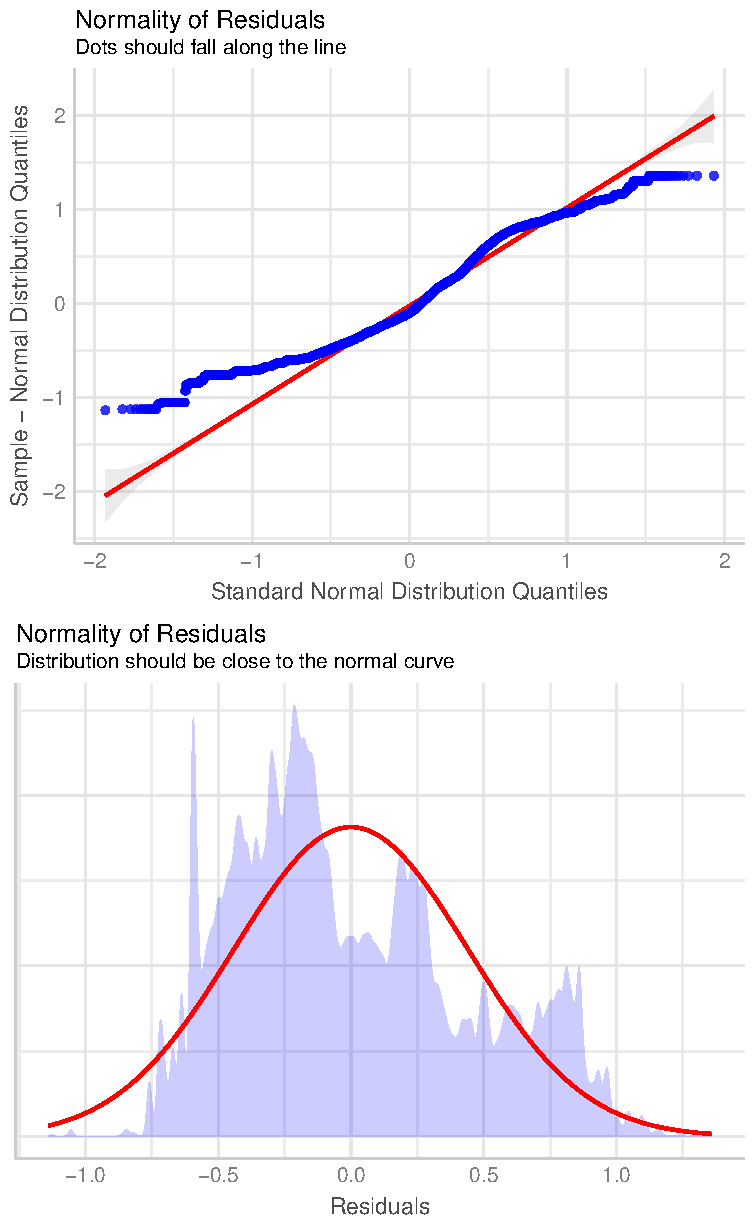
\includegraphics[scale=0.7]{Supporting/Chapter3/Figures/Diagnostics/Diag_model4b}
\caption[Diagnostic plots for Model 4b]{\textbf{Diagnostic plots for \underline{Model 4b},} obtained using the `performance' R package \citep{performance}.}
\label{SI3_F15}
\end{figure}

% Model 5a class
\begin{figure}[h!]
\centering
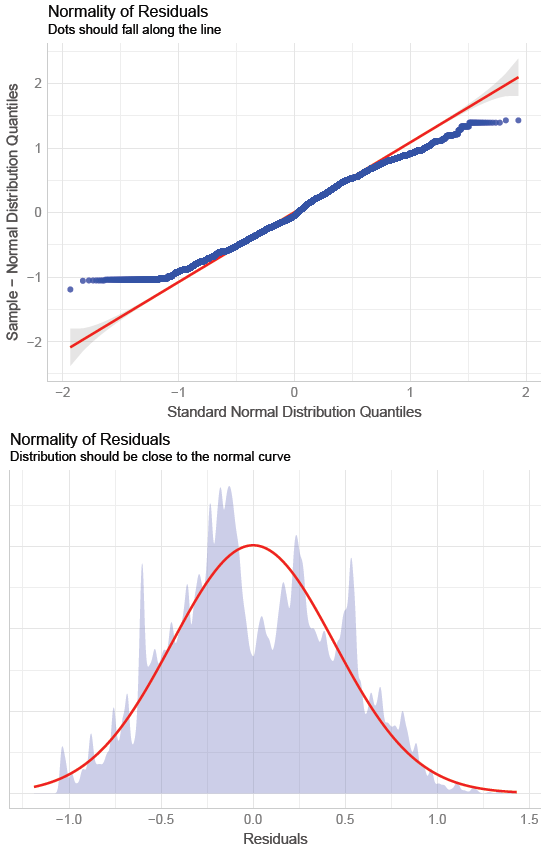
\includegraphics[scale=0.6]{Supporting/Chapter3/Figures/Diagnostics/Model5a_diag}
\caption[Diagnostic plots for Model 5a]{\textbf{Diagnostic plots for \underline{Model 5a},} obtained using the `performance' R package \citep{performance}.}
\label{SI3_F16}
\end{figure}


% Model 5b
\begin{figure}[h!]
\centering
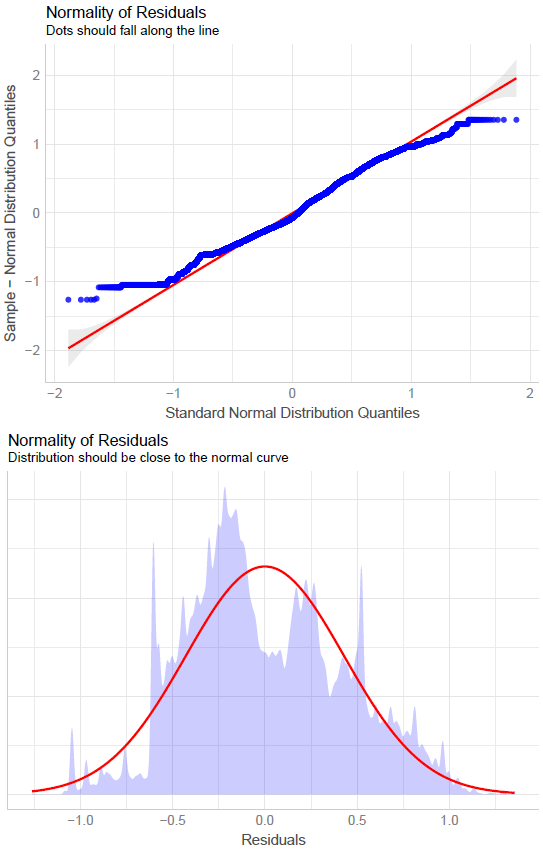
\includegraphics[scale=0.6]{Supporting/Chapter3/Figures/Diagnostics/Model5b_diag}
\caption[Diagnostic plots for Model 5b]{\textbf{Diagnostic plots for \underline{Model 5b},} obtained using the `performance' R package \citep{performance}.}
\label{SI3_F17}
\end{figure}

\newpage
\clearpage

\section{Model robustness}

%%% Model across all verts

%% effects across all verts (complete subset)
\begin{figure}[h!]
\centering
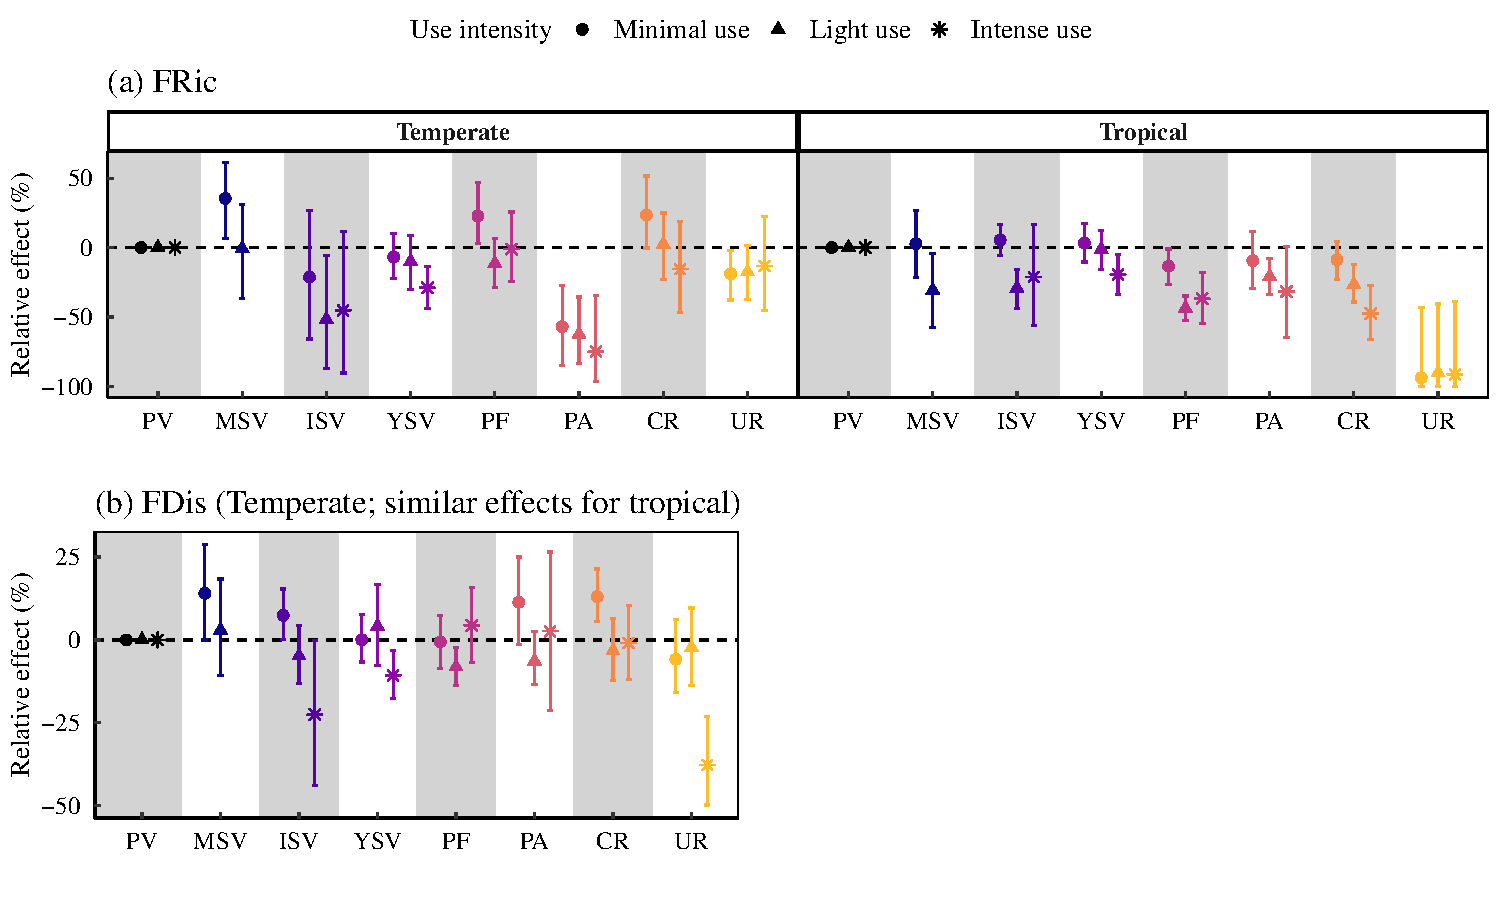
\includegraphics[scale=0.7]{Supporting/Chapter3/Figures/SI_Figure18}
\caption[Effects of land use, use intensity and region on FRic (a) and FDis (b) across vertebrates, for the subset of species with complete trait data]{\textbf{Effects of land use, use intensity and region on FRic (a) and FDis (b) across vertebrates, for the subset of species with complete trait data (i.e., excluding species with less than 100\% trait completeness).} Effects are plotted as a \% difference relative to the reference land use (primary vegetation, PV). For FRic, we fitted Model 1a (see main text), which included the effects of land use, use intensity and region, as well as interactions between land use and use intensity and between land use and region. For FDis, we fitted Model 1b (see main text), which included effects of land use, use intensity and region, and interactions between land use and use intensity. Error bars represent 95\% confidence intervals. MSV: mature secondary vegetation; ISV: intermediate secondary vegetation; YSV: young secondary vegetation; PF: plantation forest; PA: pasture; CR: cropland; UR: urban. Effects for Intense use in MSV could not be estimated as there weren’t enough sampled sites.}
\label{SI3_F18}
\end{figure}

%% robustness to trait omission
\begin{figure}[h!]
\centering
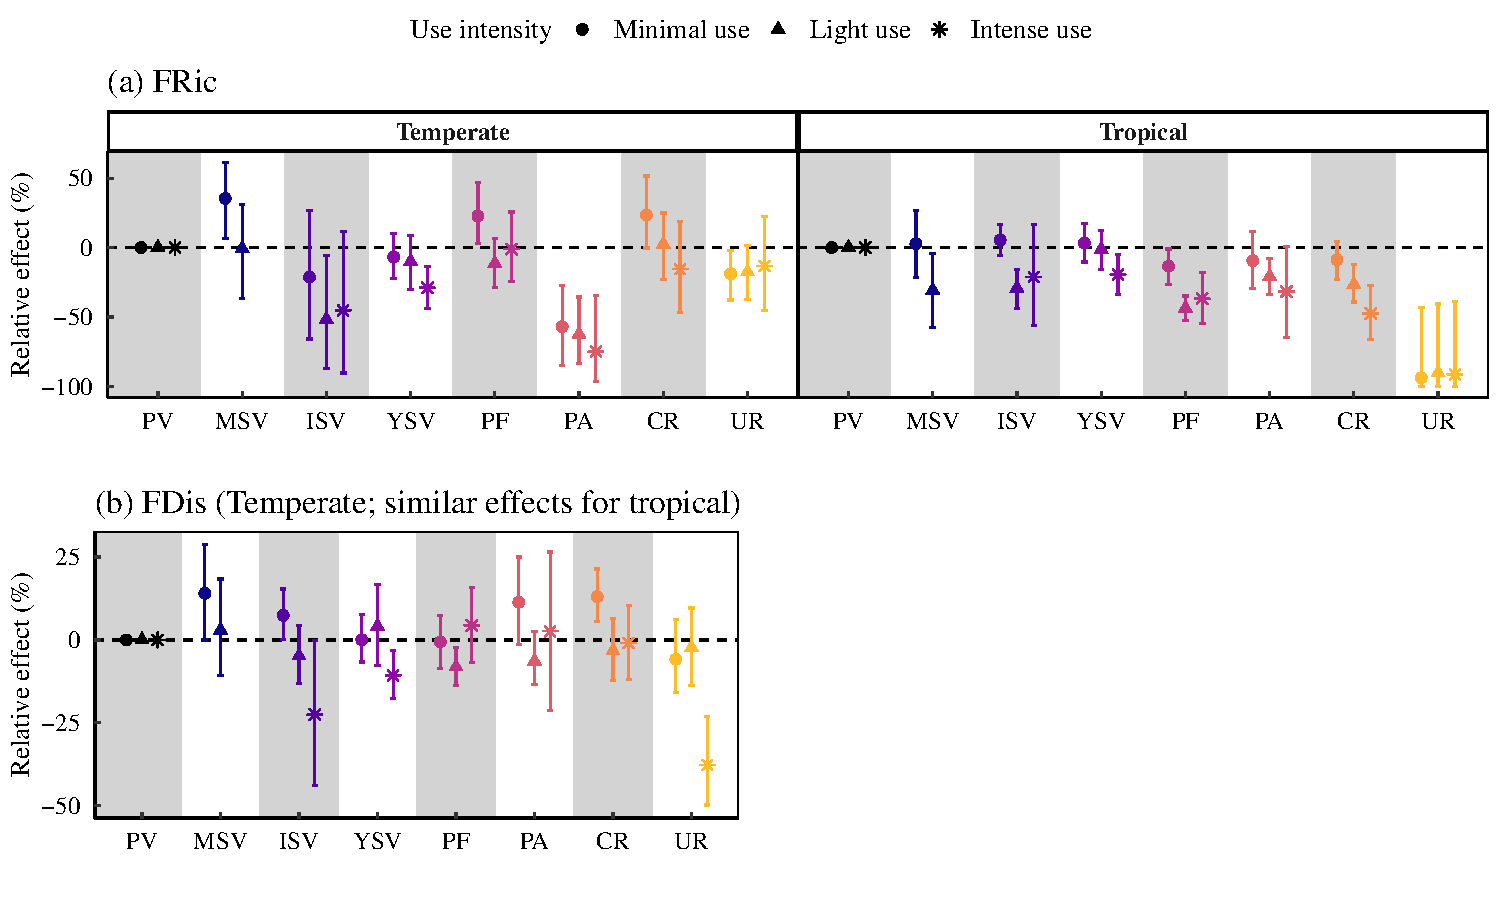
\includegraphics[scale=0.7]{Supporting/Chapter3/Figures/SI_Figure19}
\caption[Effects of land use, use intensity and region on FRic (a) and FDis (b), for the subset of species with complete trait data, with geographical range size as an additional trait]{\textbf{Effects of land use, use intensity and region on FRic (a) and FDis (b), for the subset of species with complete trait data (i.e., excluding species with less than 100\% trait completeness), with geographical range size as an additional trait considered in the calculation of functional diversity metrics.} Effects are plotted as a \% difference relative to the reference land use (primary vegetation, PV). For FRic, we fitted Model 1a (see main text), which included the effects of land use, use intensity and region, as well as interactions between land use and use intensity and between land use and region. For FDis, we fitted Model 1b (see main text), which included effects of land use, use intensity and region, and interactions between land use and use intensity. Error bars represent 95\% confidence intervals. MSV: mature secondary vegetation; ISV: intermediate secondary vegetation; YSV: young secondary vegetation; PF: plantation forest; PA: pasture; CR: cropland; UR: urban. Effects for Intense use in MSV could not be estimated as there weren’t enough sampled sites.}
\label{SI3_F19}
\end{figure}

%% robustness to variation across imputed values
\begin{figure}[h!]
\centering
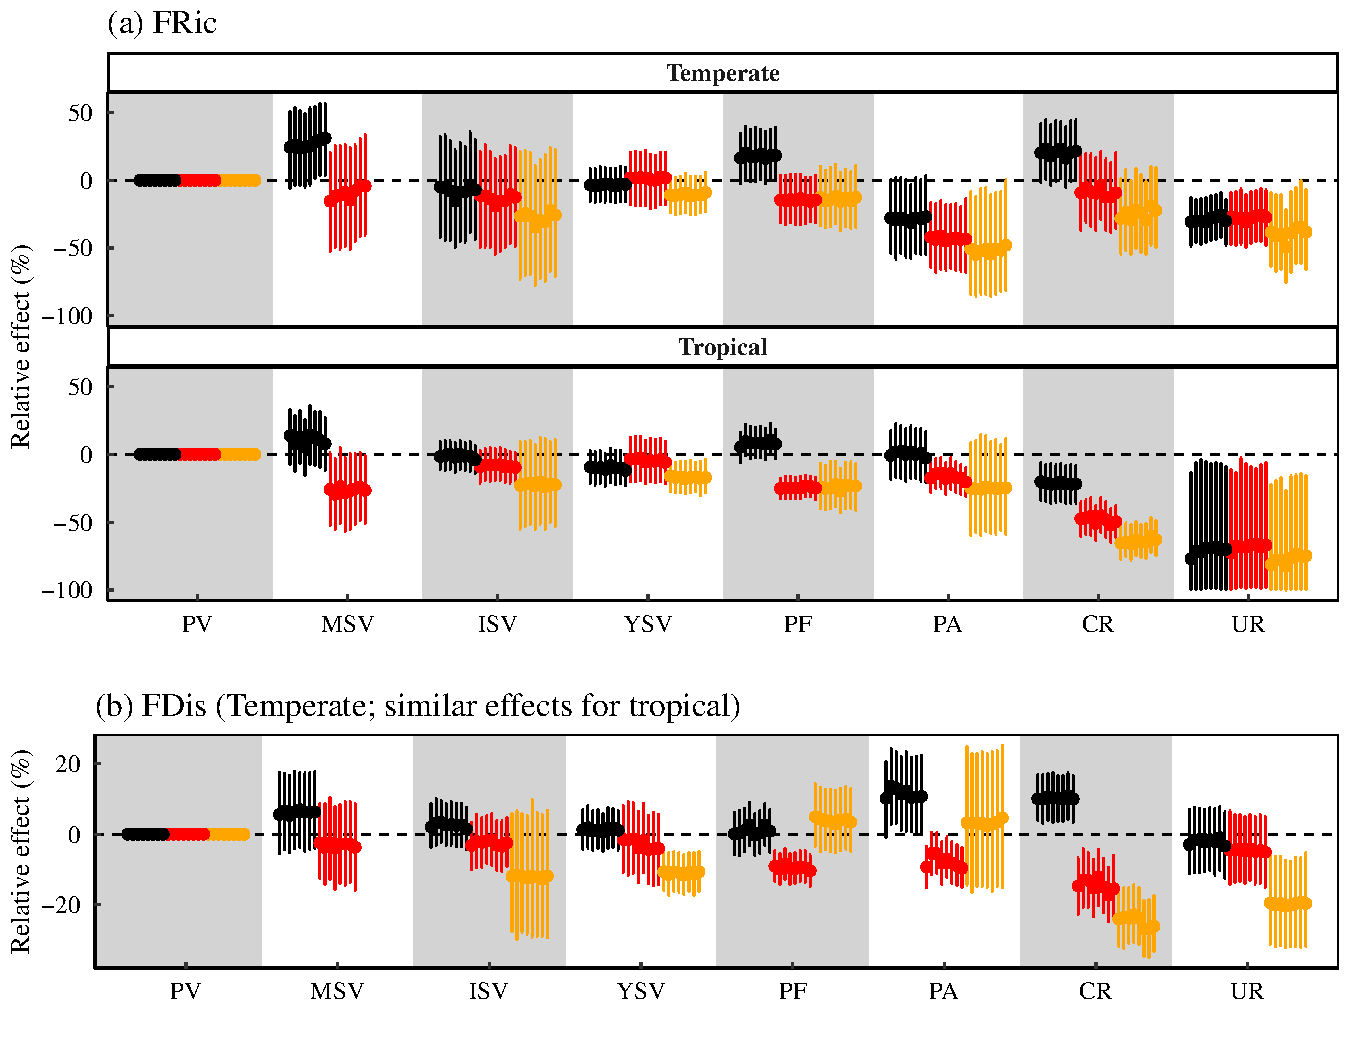
\includegraphics[scale=0.7]{Supporting/Chapter3/Figures/Figure_SI_20}
\caption[Effects of land use and use intensity on FRic (a) and FDis (b), obtained when calculating FRic and FDis with each set of imputed traits]{\textbf{Effects of land use and use intensity on FRic (a) and FDis (b), obtained when calculating FRic and FDis with each set of imputed traits (eight in total).} Effects are plotted as a \% difference relative to the reference land use (primary vegetation, PV). For FRic, we fitted Model 1a (see main text), which included the effects of land use, use intensity and region, as well as interactions between land use and use intensity and between land use and region. For FDis, we fitted Model 1b (see main text), which included effects of land use, use intensity and region, and interactions between land use and use intensity. Error bars represent 95\% confidence intervals. MSV: mature secondary vegetation; ISV: intermediate secondary vegetation; YSV: young secondary vegetation; PF: plantation forest; PA: pasture; CR: cropland; UR: urban. Effects for Intense use in MSV could not be estimated as there weren’t enough sampled sites.}
\label{SI3_F20}
\end{figure}

%% robustness to resampling in primary vegetation sites
\begin{figure}[h!]
\centering
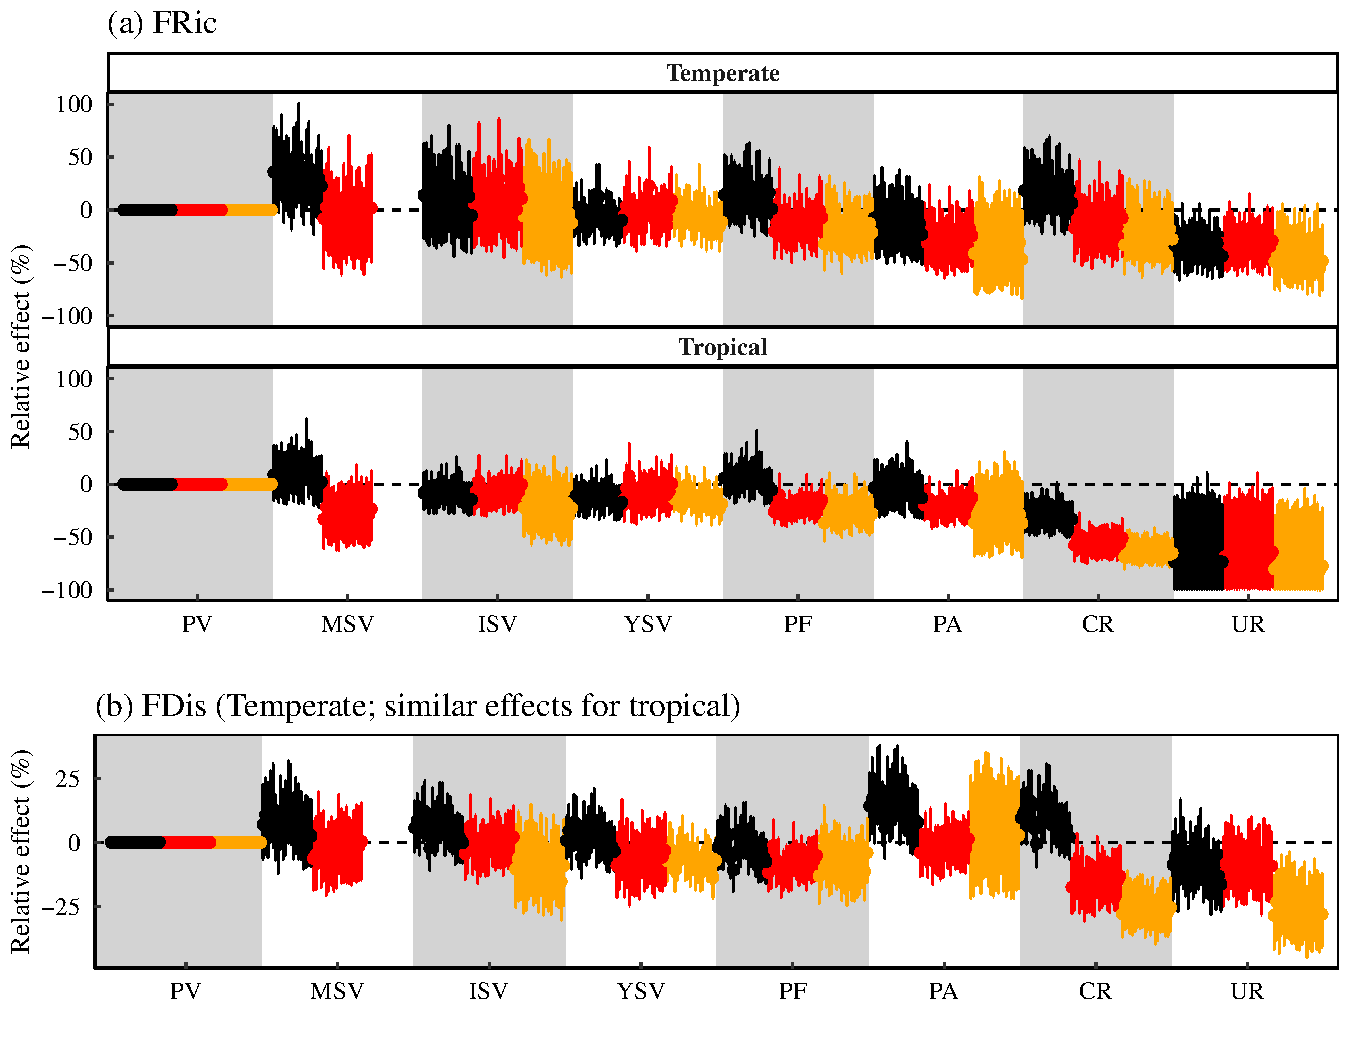
\includegraphics[scale=0.7]{Supporting/Chapter3/Figures/Figure_SI_21}
\caption[Effects of land use and use intensity on FRic (a) and FDis (b), obtained when re-sampling primary vegetation sites twenty independent times]{\textbf{Effects of land use and use intensity on FRic (a) and FDis (b), obtained when re-sampling primary vegetation sites twenty independent times.} We fixed the sample size for primary vegetation sites at 50 (see main text, Material and Methods, `Effects of land use and use intensity on FRic and FDis (hypothesis 1)'). For FRic, we fitted Model 1a (see main text), which included the effects of land use, use intensity and region, as well as interactions between land use and use intensity and between land use and region. For FDis, we fitted Model 1b (see main text), which included effects of land use, use intensity and region, and interactions between land use and use intensity. Error bars represent 95\% confidence intervals. MSV: mature secondary vegetation; ISV: intermediate secondary vegetation; YSV: young secondary vegetation; PF: plantation forest; PA: pasture; CR: cropland; UR: urban. Effects for Intense use in MSV could not be estimated as there weren’t enough sampled sites.}
\label{SI3_F21}
\end{figure}


%%% Model by class

%% effects by class(complete subset)
\begin{figure}[h!]
\centering
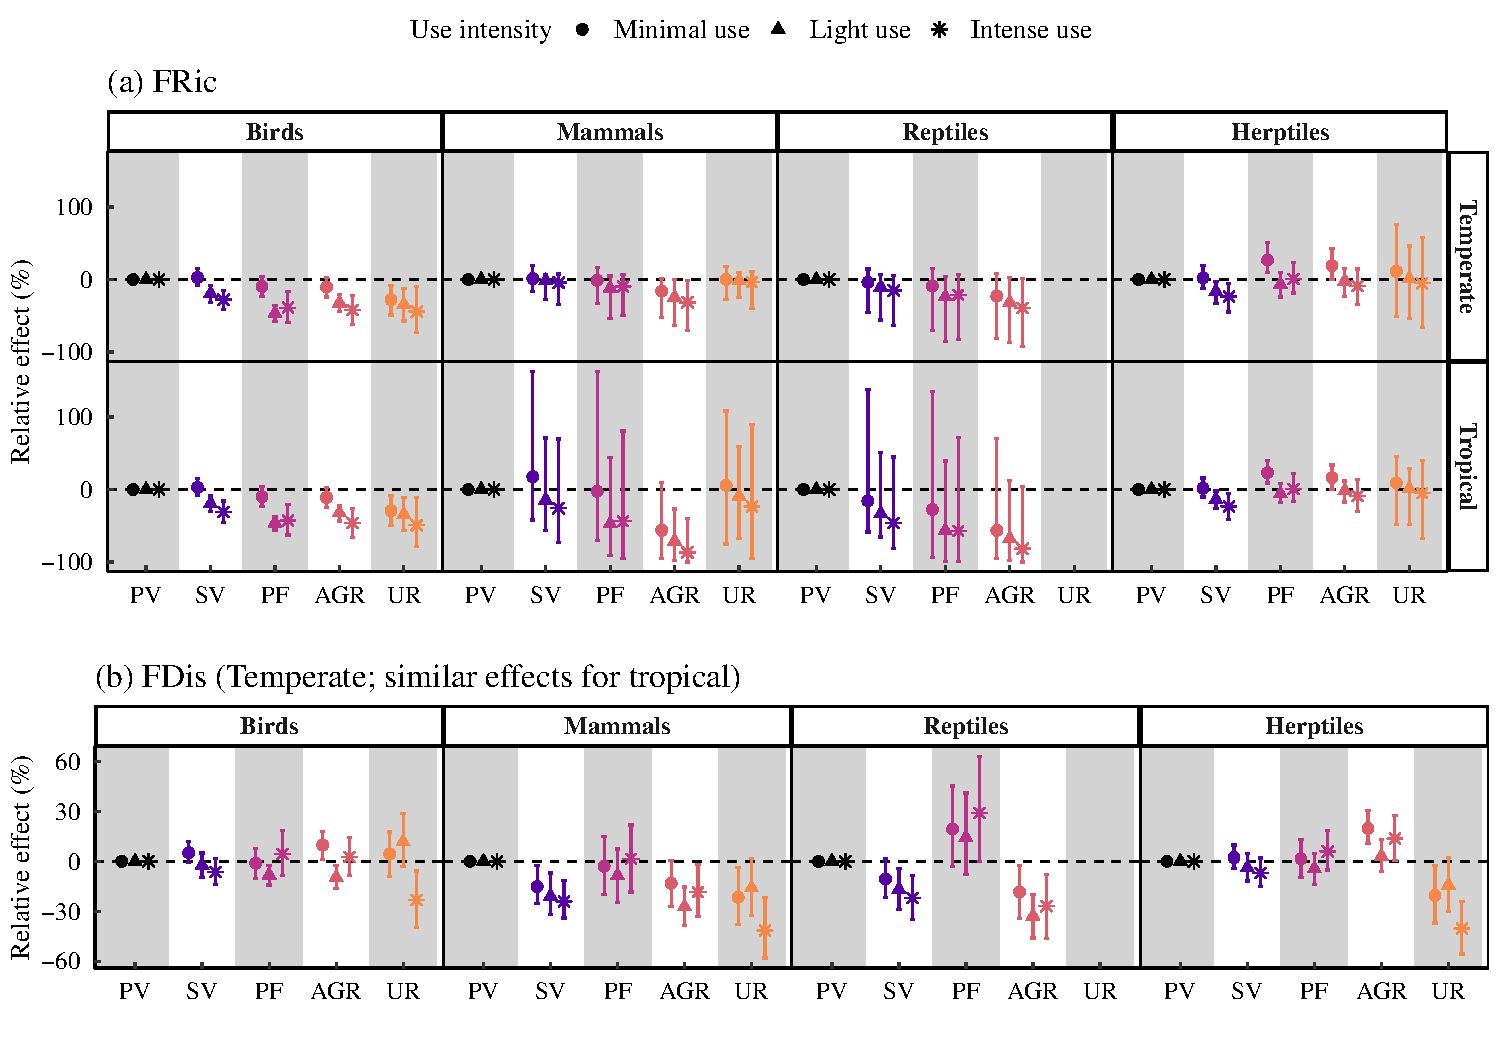
\includegraphics[scale=0.7]{Supporting/Chapter3/Figures/SI_Figure22}
\caption[Effects of land use, use intensity and taxonomic class on FRic (a) and FDis (c), for the subset of species with complete trait data]{\textbf{Effects of land use, use intensity and taxonomic class on FRic (a) and FDis (c), for the subset of species with complete trait data (i.e., excluding species with less than 100\% trait completeness).} Effects are plotted as a \% difference relative to the reference land use (primary vegetation, PV). We did not include the effects of region here as sample sizes were not large enough for some classes. For FRic, the model included the effects of land use, use intensity and class, and interactions between land use and use intensity as well as land use and class. For FDis, the model included an additional interaction between use intensity and class. Error bars represent 95\% confidence intervals. SV: secondary vegetation; PF: plantation forest; PA: pasture; CR: cropland; UR: urban. Effects for reptiles in urban land uses could not be estimated as there weren’t enough sampled sites.}
\label{SI3_F22}
\end{figure}


%% comparison 
\begin{figure}[h!]
\centering
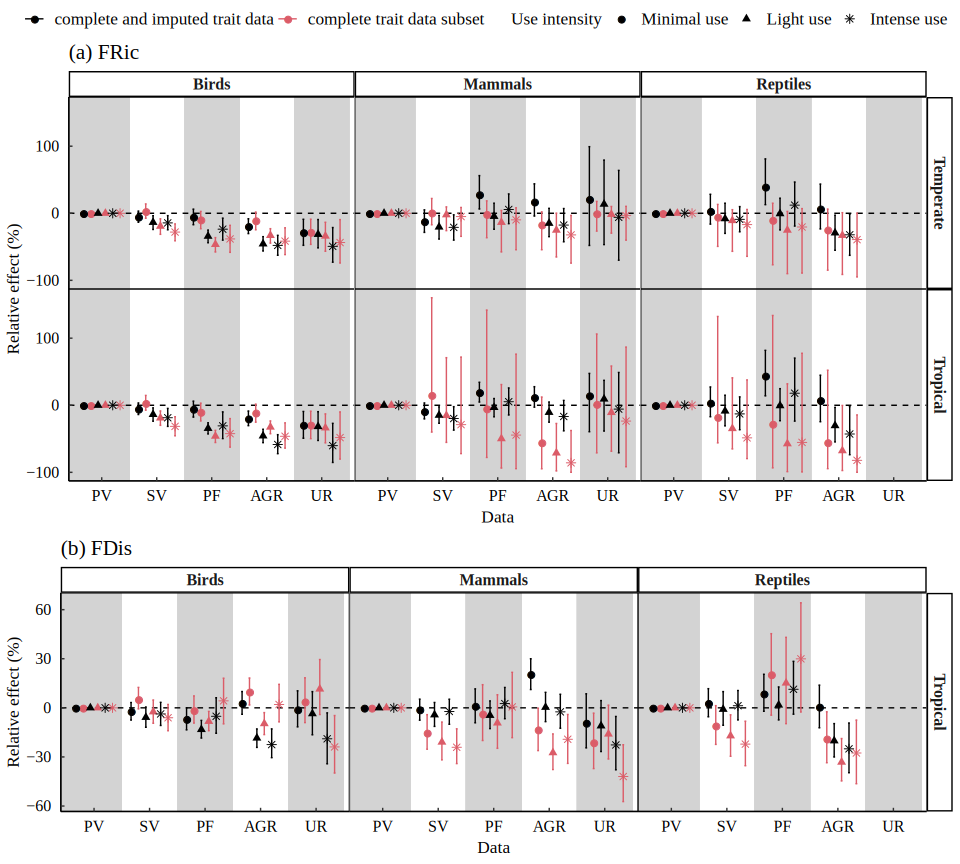
\includegraphics[scale=0.7]{Supporting/Chapter3/Figures/SI_Comparison_complete}
\caption[Effects of land use, region, use intensity and taxonomic class on FRic and FDis obtained with the imputed trait data (black points) or with the complete data subsets (red points)]{\textbf{Effects of land use, region, use intensity and taxonomic class on FRic and FDis obtained with the imputed trait data (black points) or with the complete data subsets (red points).} Effects are plotted as a \% difference relative to the reference land use (primary vegetation, PV). For FRic, we fitted Model 2a (see main text), and we fitted Model 2b for FDis. Error bars represent 95\% confidence intervals. SV: secondary vegetation; PF: plantation forest; AGR:agricultural (cropland and pasture); UR: urban. Effects for reptiles in urban land uses could not be estimated as there weren’t enough sampled sites.}
\label{SI3_F23}
\end{figure}

%% robustness to imputation variability
\begin{figure}[h!]
\centering
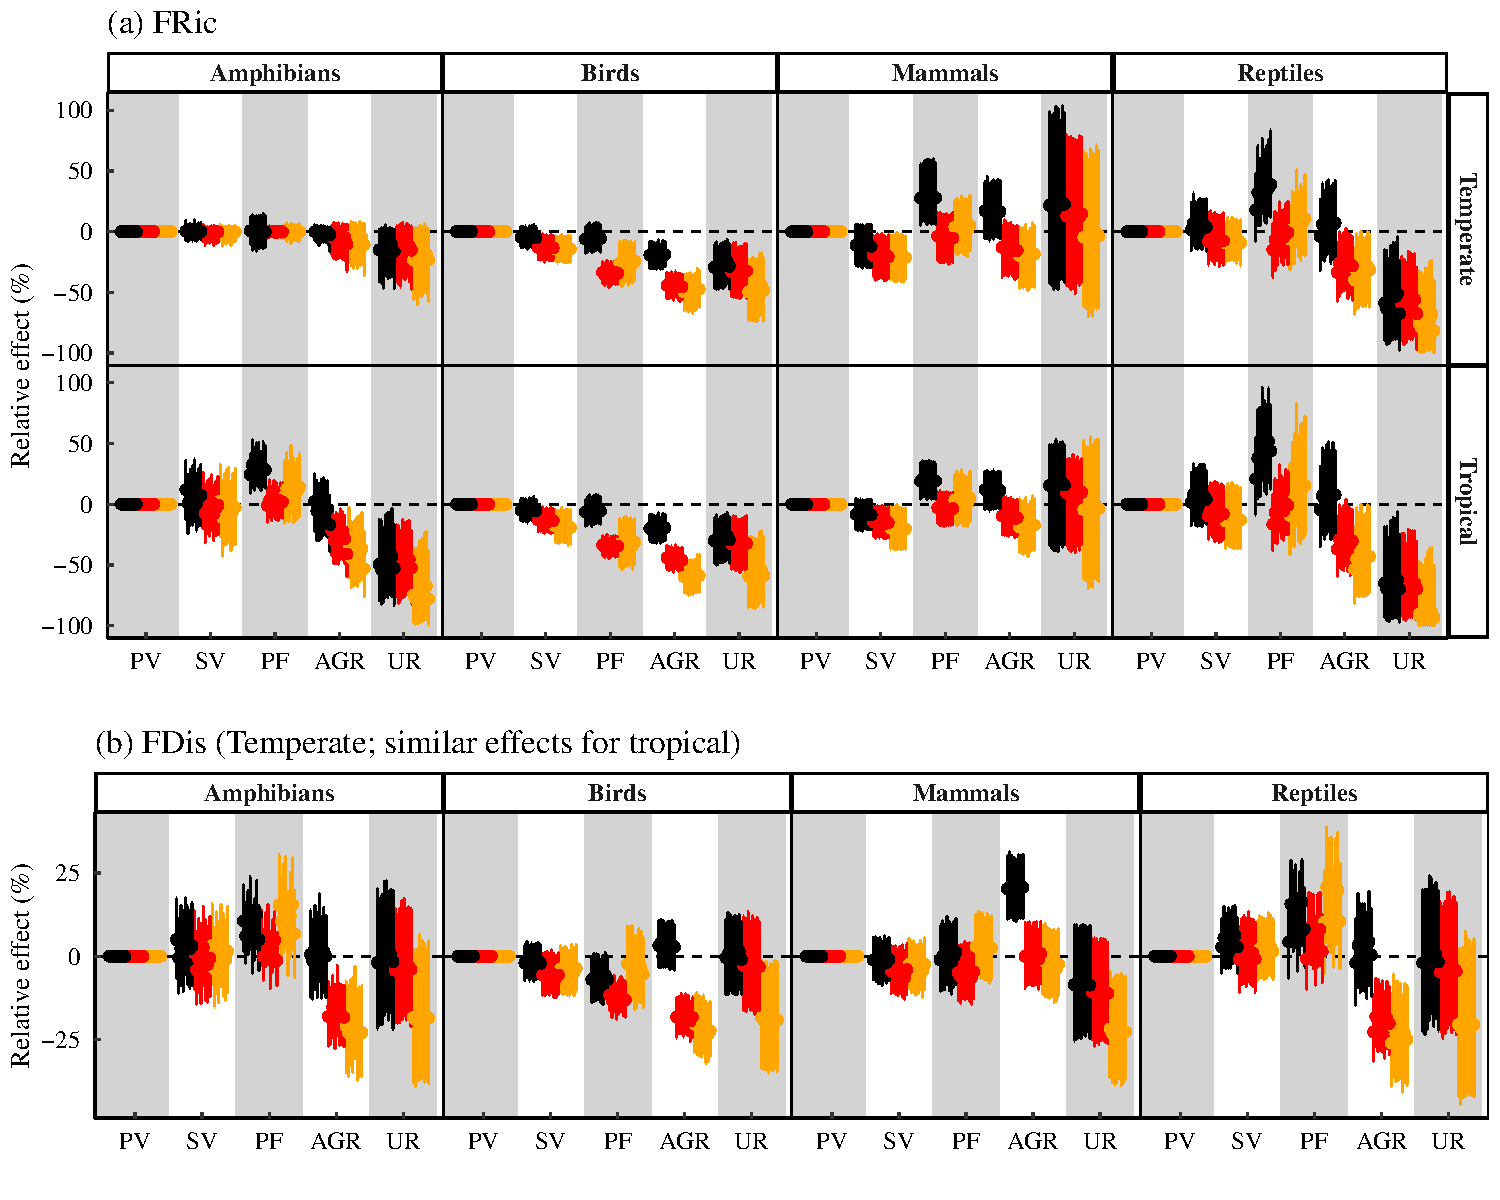
\includegraphics[scale=0.7]{Supporting/Chapter3/Figures/Figure_SI_23}
\caption[Effects of land use, region, use intensity and taxonomic class on FRic and FDis, obtained when calculating FRic and FDis with each set of imputed traits]{\textbf{Effects of land use, region, use intensity and taxonomic class on FRic and FDis, obtained when calculating FRic and FDis with each set of imputed traits (eight in total).} Effects are plotted as a \% difference relative to the reference land use (primary vegetation, PV). For FRic, we fitted Model 2a (see main text), and Model 2b for FDis. Error bars represent 95\% confidence intervals. SV: secondary vegetation; PF: plantation forest; AGR:agricultural (cropland and pasture); UR: urban. Effects for reptiles in urban land uses could not be estimated as there weren’t enough sampled sites.}
\label{SI3_F24}
\end{figure}


\newpage
\begin{comment}
%% sensitivity fig 3
\begin{figure}[h!]
\centering
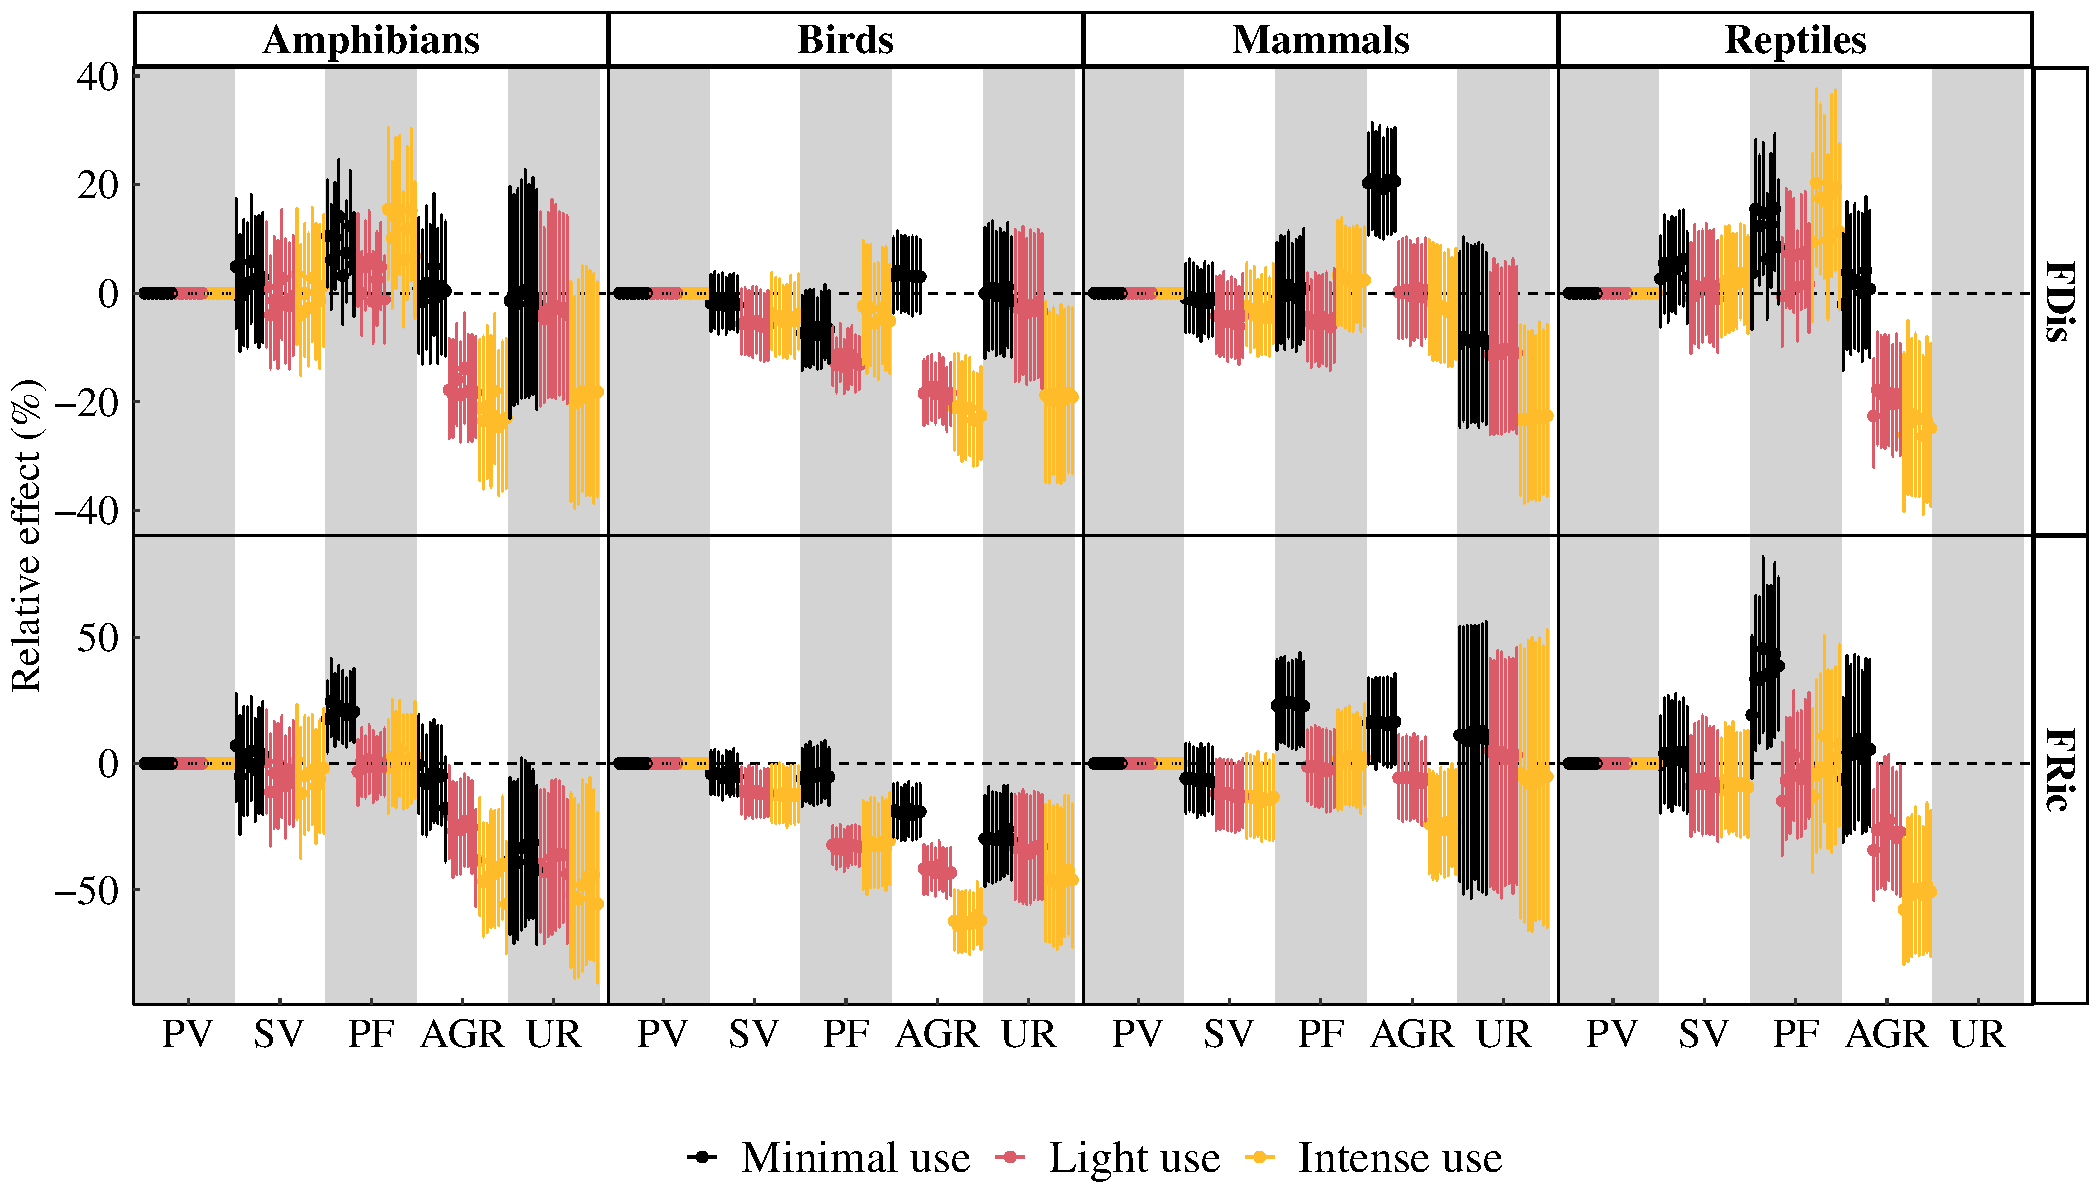
\includegraphics[scale=0.5]{Supporting/Chapter3/Figures/SI_sensitivity_fig3bis}
\caption[Effects of land use, use intensity and taxonomic class on FRic and FDis, obtained when calculating FRic and FDis with each set of imputed traits]{\textbf{Effects of land use, use intensity and taxonomic class on FRic and FDis, obtained when calculating FRic and FDis with each set of imputed traits (eight in total).} Effects are plotted as a \% difference relative to the reference land use (primary vegetation, PV). Error bars represent 95\% confidence intervals. SV: secondary vegetation; PF: plantation forest; PA: pasture; CR: cropland; UR: urban. Effects for reptiles in urban land uses could not be estimated as there weren’t enough sampled sites.}
\label{}
\end{figure}
\end{comment}



\pagebreak
\clearpage



\begin{comment}
%% model summary: range size ~ habitat breadth + class

% Table created by stargazer v.5.2.2 by Marek Hlavac, Harvard University. E-mail: hlavac at fas.harvard.edu
% Date and time: Fri, May 21, 2021 - 13:33:14
\begin{table}[!htbp] \centering 
  \caption{} 
  \label{} 
\begin{tabular}{@{\extracolsep{5pt}}lc} 
\\[-1.8ex]\hline 
\hline \\[-1.8ex] 
 & \multicolumn{1}{c}{\textit{Dependent variable:}} \\ 
\cline{2-2} 
\\[-1.8ex] & logrs \\ 
\hline \\[-1.8ex] 
 Constant & 7.127$^{***}$ (6.536, 7.718) \\ 
  sqrthb & 2.173$^{***}$ (1.890, 2.455) \\ 
  I(sqrthb$\hat{\mkern6mu}$2) & $-$0.101$^{***}$ ($-$0.132, $-$0.070) \\ 
  ClassBirds & 4.007$^{***}$ (3.421, 4.592) \\ 
  ClassMammals & 4.607$^{***}$ (3.887, 5.326) \\ 
  ClassReptiles & 3.007$^{***}$ (2.069, 3.945) \\ 
  sqrthb:ClassBirds & $-$0.747$^{***}$ ($-$0.981, $-$0.512) \\ 
  sqrthb:ClassMammals & $-$0.817$^{***}$ ($-$1.114, $-$0.519) \\ 
  sqrthb:ClassReptiles & $-$0.703$^{***}$ ($-$1.111, $-$0.296) \\ 
 \hline \\[-1.8ex] 
Observations & 4,099 \\ 
R$^{2}$ & 0.258 \\ 
Adjusted R$^{2}$ & 0.256 \\ 
Residual Std. Error & 1.951 (df = 4090) \\ 
F Statistic & 177.656$^{***}$ (df = 8; 4090) \\ 
\hline 
\hline \\[-1.8ex] 
\textit{Note:}  & \multicolumn{1}{r}{$^{*}$p$<$0.1; $^{**}$p$<$0.05; $^{***}$p$<$0.01} \\ 
\end{tabular} 
\end{table}

%% model summary -- home range versus habitat breadth
% Table created by stargazer v.5.2.2 by Marek Hlavac, Harvard University. E-mail: hlavac at fas.harvard.edu
% Date and time: Fri, May 21, 2021 - 13:44:20
\begin{table}[!htbp] \centering 
  \caption{} 
  \label{} 
\begin{tabular}{@{\extracolsep{5pt}}lc} 
\\[-1.8ex]\hline 
\hline \\[-1.8ex] 
 & \multicolumn{1}{c}{\textit{Dependent variable:}} \\ 
\cline{2-2} 
\\[-1.8ex] & logHR \\ 
\hline \\[-1.8ex] 
 Constant & $-$3.441$^{***}$ ($-$5.006, $-$1.875) \\ 
  sqrthb & 0.854$^{***}$ (0.308, 1.401) \\ 
 \hline \\[-1.8ex] 
Observations & 126 \\ 
R$^{2}$ & 0.070 \\ 
Adjusted R$^{2}$ & 0.063 \\ 
Residual Std. Error & 3.428 (df = 124) \\ 
F Statistic & 9.400$^{***}$ (df = 1; 124) \\ 
\hline 
\hline \\[-1.8ex] 
\textit{Note:}  & \multicolumn{1}{r}{$^{*}$p$<$0.1; $^{**}$p$<$0.05; $^{***}$p$<$0.01} \\ 
\end{tabular} 
\end{table} 

\end{comment}

\newpage
\clearpage
\section{Model robustness -- time since land-use conversion}
Time since land-use conversion could have important impacts on assemblage composition and thus, on local functional diversity. We did not investigate these effects because PREDICTS contained data on time since land-use conversion only for about 22\% of the sites, considerably reducing samples sizes. Here, we investigated whether our results are likely robust to the inclusion of time since land-use conversion using the subset of sites for which  time since land-use conversion was provided. To this end, we find the best-fitting models explaining FRic and FDis, using backwards stepwise selection, starting with complete models that include the effects of land use, time since land-use conversion, region, use intensity (for FRic only) and all two-way interactions among these predictors. 

\begin{itemize}
\item For FRic, the best-fitting model includes the main effects of land use and time since land-use conversion, but no interaction between these predictors. The model’s summary (Table S6) show that time since conversion has a significant negative effect on FRic, but the relationship between FRic and time since land-use conversion is similar in different land uses (as there are no interactions between land use and time since conversion, such that the slopes are similar in different land uses, and so the rate at which FRic decreases with time is similar in different land uses). The intercept is only different for urban land uses (significantly lower). Thus, based on this data subset, we expect time since land-use conversion to have a similar effect in different land uses. 
\vspace{0.3cm}

\begin{table}[!htbp] \centering 
  \caption[Summary of the model explaining FRic by land use and time since land-use conversion, fitted on the subset of data for which we have information on time since land-use conversion]{Summary of the model explaining FRic by land use and time since land-use conversion, fitted on the subset of data for which we have information on time since land-use conversion.} 
  \label{SI3_Table6} 
\begin{tabular}{@{\extracolsep{5pt}} lccc} 
\\[-1.8ex]\hline 
\hline \\[-1.8ex] 
 & Estimate & Std. Error & t value \\ 
\hline \\[-1.8ex] 
Intercept: Primary vegetation & $1.156$ & $0.073$ & $15.921$ \\ 
Mature secondary vegetation & $0.178$ & $0.093$ & $1.907$ \\ 
Intermediate secondary vegetation & $0.018$ & $0.072$ & $0.249$ \\ 
Young secondary vegetation & $$-$0.078$ & $0.051$ & $$-$1.532$ \\ 
Plantation forest & $$-$0.018$ & $0.082$ & $$-$0.224$ \\ 
Pasture & $$-$0.005$ & $0.093$ & $$-$0.054$ \\ 
Cropland & $0.133$ & $0.152$ & $0.875$ \\ 
Urban & $$-$0.316$ & $0.133$ & $$-$2.368$ \\ 
log\_Years & $$-$0.094$ & $0.021$ & $$-$4.566$ \\ 
\hline \\[-1.8ex] 
\end{tabular} 
\end{table} 

We then compare this model’s predictions with a simpler model that doesn’t account for time since land-use conversion (FRic  $\thicksim$ Land use). The predictions (Fig. S25) show that including time since land-use conversion doesn’t bias our results, as we find a similar significant effect with both models in urban land uses, and elsewhere the effects are congruent. Thus, given this data subset, we argue that our results are robust to the inclusion of time since land-use conversion.
%\vspace(0.5cm)

\begin{figure}[h!]
\centering
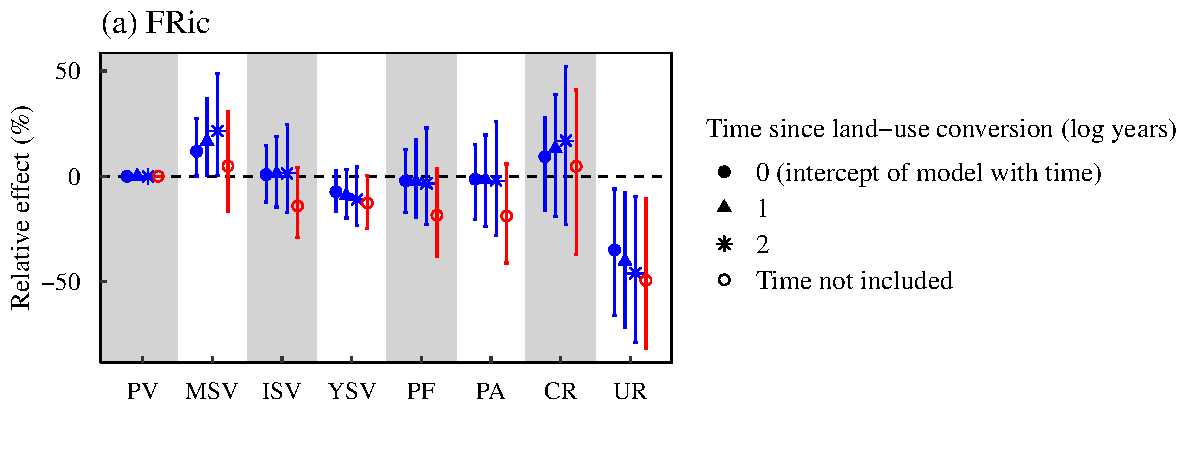
\includegraphics[scale=0.7]{Supporting/Chapter3/Figures/SI_time_since_conv_FRic}
\caption[Effects of land use on FRic for the model that includes time since land-use conversion (blue points) versus the model that doesn't take time since land-use conversion into account (red points)]{\textbf{Effects of land use on FRic for the model that includes time since land-use conversion (blue points) versus the model that doesn't take time since land-use conversion into account (red points)}.}
\label{SI3_F25}
\end{figure}


\item For FDis, the best-fitting model includes the main effects of land use, time since land-use conversion as well as interactions between land use and time since land-use conversion (we didn't consider use intensity in the starting model because of sample size issues). Nevertheless, the main effect of time since land-use conversion is not significant (Table S7), and the relationship between time since land-use conversion and FDis is not significant in most land uses (except for plantation forest). Thus, we argue the available data don’t allow us to properly investigate the relationship between time since land-use conversion and FDis.

\vspace{0.3cm}
\begin{table}[!htbp] \centering 
  \caption[Summary of the model explaining FDis by land use and time since land-use conversion, fitted on the subset of data for which we have information on time since land-use conversion]{Summary of the model explaining FDis by land use and time since land-use conversion, fitted on the subset of data for which we have information on time since land-use conversion.} 
  \label{SI3_Table7} 
\begin{tabular}{@{\extracolsep{5pt}} lccc} 
\\[-1.8ex]\hline 
\hline \\[-1.8ex] 
 & Estimate & Std. Error & t value \\ 
\hline \\[-1.8ex] 
Intercept: Primary vegetation & $0.366$ & $0.011$ & $32.219$ \\ 
Mature secondary vegetation & $0.032$ & $0.055$ & $0.577$ \\ 
Intermediate secondary vegetation & $$-$0.015$ & $0.050$ & $$-$0.298$ \\ 
Young secondary vegetation & $0.020$ & $0.015$ & $1.386$ \\ 
Plantation forest & $0.074$ & $0.023$ & $3.213$ \\ 
Pasture & $$-$0.017$ & $0.048$ & $$-$0.346$ \\ 
Cropland & $$-$0.013$ & $0.042$ & $$-$0.317$ \\ 
Urban & $0.031$ & $0.054$ & $0.573$ \\ 
log\_Years & $$-$0.004$ & $0.004$ & $$-$1.186$ \\ 
Mature secondary vegetation:log\_Years & $$-$0.005$ & $0.015$ & $$-$0.335$ \\ 
Intermediate secondary vegetation:log\_Years & $0.011$ & $0.016$ & $0.650$ \\ 
Young secondary vegetation:log\_Years & $$-$0.008$ & $0.007$ & $$-$1.170$ \\ 
Plantation forest:log\_Years & $$-$0.023$ & $0.007$ & $$-$3.077$ \\ 
Pasture:log\_Years & $0.010$ & $0.015$ & $0.688$ \\ 
Cropland:log\_Years & $0.007$ & $0.012$ & $0.620$ \\ 
Urban:log\_Years & $$-$0.016$ & $0.022$ & $$-$0.714$ \\ 
\hline \\[-1.8ex] 
\end{tabular} 
\end{table} 

\end{itemize}

